\documentclass[xcolor={usenames,dvipsnames}]{beamer}
\usepackage[utf8]{inputenc}
\usepackage[english]{babel}

% -- Including some standard packages --
\usepackage{graphicx}
\usepackage{soul}
\usepackage{hyperref}
\usepackage{colortbl}
\usepackage{dsfont}
\usepackage{soul}

% -- Choosing theme --

\usetheme{Boadilla}
\usecolortheme{spruce}
\setbeamercolor{alerted text}{fg=purple} % Making alerted text non-red

% Tikz
\usepackage{tikz,tikz-3dplot,tikz-cd,tkz-tab,tkz-euclide,pgf,pgfplots}
\usetikzlibrary{matrix,positioning,fit,backgrounds,intersections}

% -- Cross signs --
\usepackage{pifont} % http://ctan.org/pkg/pifont
\newcommand{\cmark}{\ding{51}}%
\newcommand{\xmark}{\ding{55}}%
\newcommand{\xopt}{\ding{48}}%

% -- Custom commands --
\DeclareMathOperator*{\argmax}{arg\,max}
\DeclareMathOperator*{\argmin}{arg\,min}

\title[Introduction to ZK]{\textbf{Introduction to Zero-Knowledge Proofs}}
\author{Distributed Lab}
\date{August 22, 2024}
\titlegraphic{
    
\includegraphics[width=\textwidth]{images/banner_wide.png}
}

\expandafter\def\expandafter\insertshorttitle\expandafter{%
  \insertshorttitle\hfill%
  \insertframenumber\,/\,\inserttotalframenumber}

\AtBeginSection[]{
  \begin{frame}
  \vfill
  \centering
  \begin{beamercolorbox}[sep=8pt,center,shadow=true,rounded=true]{title}
    \usebeamerfont{title}\insertsectionhead\par%
  \end{beamercolorbox}
  \vfill
  \end{frame}
}

\begin{document}
	\frame {
		\titlepage
	}
 
	\begin{frame}{Plan}
        \tableofcontents
    \end{frame}

	\section{Introduction}

    \subsection{Classical Proofs}
    \begin{frame}{Classical Proofs}
        \begin{columns}
            % Description
            \begin{column}{0.6\textwidth}
                \begin{itemize}
                    \item First proofs you have probably encountered were \textbf{geometry proofs}. 
                    \item You were given \textbf{axioms} and you can prove certain \textbf{statements} $x$ using them.
                    \item The proof $\pi$ is a sequence of logical steps that lead from axioms to the statement. Essentially, you have a witness $w$ that proves the statement.
                    \item Your teacher is the \textbf{verifier} $\mathcal{V}$ who checks your proof, while you are the \textbf{prover} $\mathcal{P}$.
                    \item This is a \textbf{classical proof} and in a sense, it is a \textbf{non-interactive proof}.
                \end{itemize}
            \end{column}
            % Column 2    
            \begin{column}{0.4\textwidth}
                \begin{figure}
                \centering
                    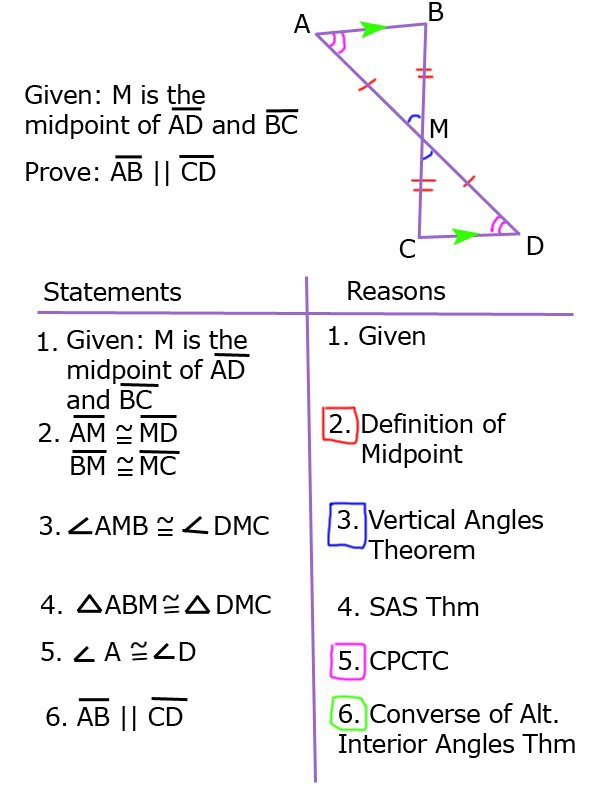
\includegraphics[width=1.0\textwidth]{images/lecture_6/geometry-proof.jpg}
                    \caption{Geometry proof.}
                \end{figure}
            \end{column}
            \end{columns}
    \end{frame}

    \begin{frame}{Motivation}
        \begin{alertblock}{Note}
            However, we cannot use such proofs in the digital world. 
            
            \begin{itemize}
                \item Proofs must be verified by computers. Therefore, we need to develop \textbf{mathematic framework} to be able to program them.
                \item This leads to the question: what is \textbf{statement}? What is \textbf{proof}? What is \textbf{witness}? How to formally define them?
                \item We need to formalize these concepts.
            \end{itemize}
        \end{alertblock}

        \begin{figure}
            \centering
            
\includegraphics[width=0.25\textwidth]{images/lecture_6/thonk.png}
            \caption{Hmm\ldots}
        \end{figure}
    \end{frame}

    \subsection{Goal of the course}
    \begin{frame}{The most basic setting}
        \begin{itemize}
            \item We have a \textbf{prover} $\mathcal{P}$ and a \textbf{verifier} $\mathcal{V}$.
            \item Prover $\mathcal{P}$ wants to prove some statement $x$ to the verifier.
            \item Prover $\mathcal{P}$ has a \textbf{witness} $w$ that contains all necessary information to prove the statement $x$. He sends $\pi$ as a proof.
            \item Verifier $\mathcal{V}$ wants to be convinced that the statement $x$ is true.
        \end{itemize}

        \begin{figure}
            \centering
            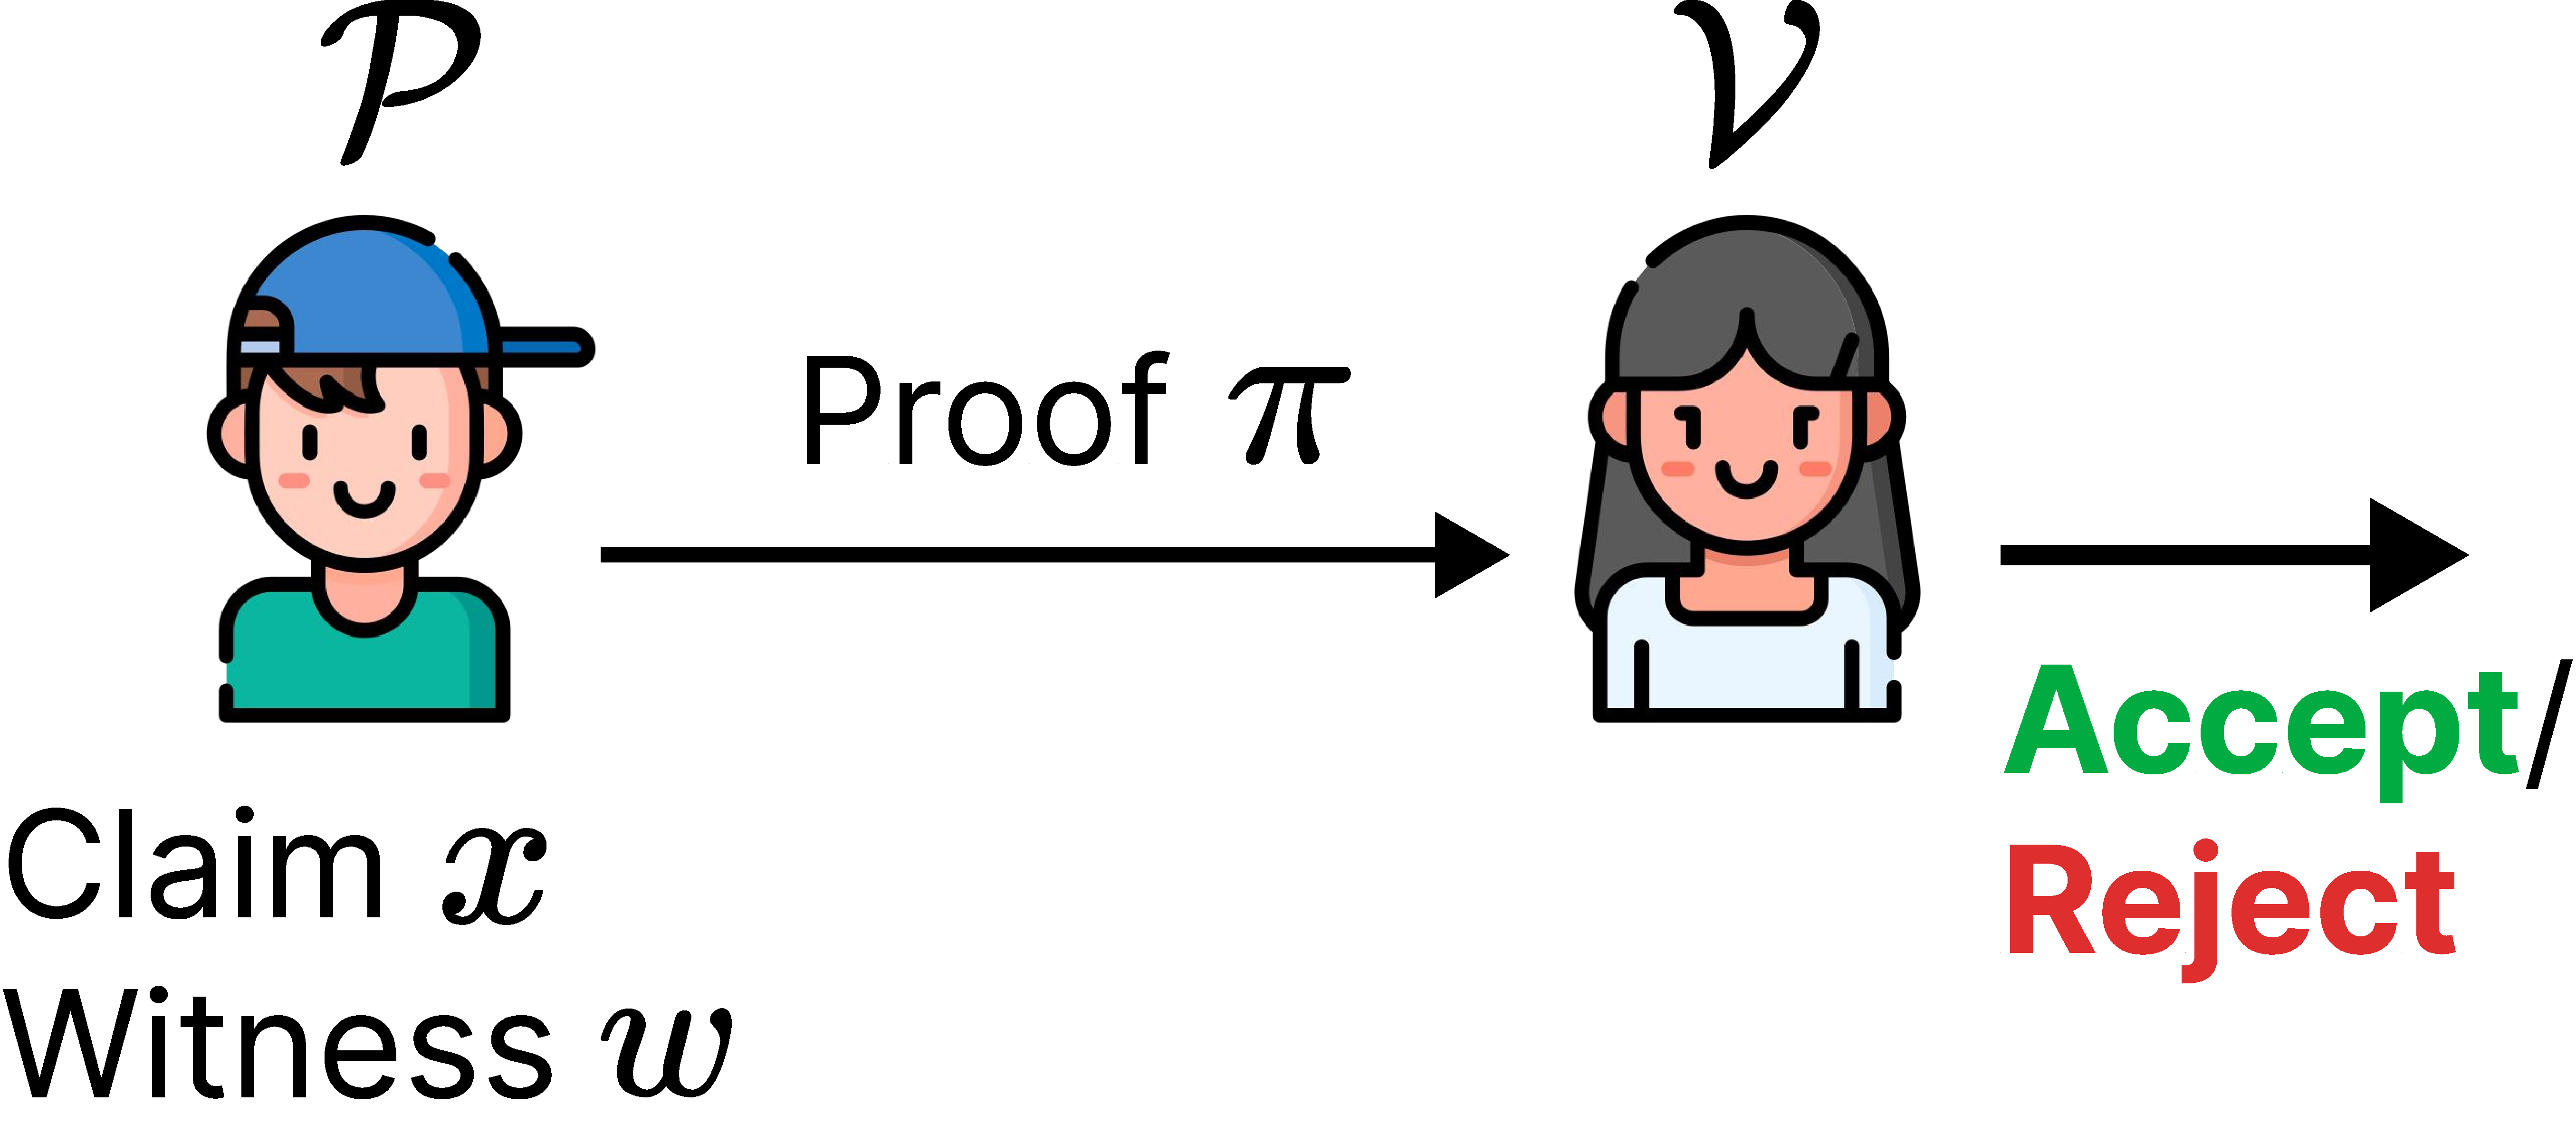
\includegraphics[width=0.7\textwidth]{images/lecture_6/setup.pdf}
            \caption{Typical setup for cryptographic proofs.}
        \end{figure}
    \end{frame}

    \begin{frame}{The Goal of SNARKs, STARKs etc.}
        We will try to solve the following problems:
        \begin{itemize}
            \item \textbf{Completeness:} If $x$ is true, $\pi$ proofs the statement.
            \item \textbf{Soundness:} If $x$ is false, the prover $\mathcal{P}$ should not be able to convince the verifier $\mathcal{V}$ via any $\pi^*$.
            \item \textbf{Zero-knowledge:} $\pi$ does not reveal anything about $w$.
            \item \textbf{Argument of knowledge:} Sometimes, the prover $\mathcal{P}$ should convince the verifier $\mathcal{V}$ that besides $x$ is true, he \textbf{knows} the witness $w$.
            \item \textbf{Succinctness:} The proof should be short, ideally polylogarithmic in the size of the statement ($\pi = \mathsf{polylog}(|x|)$) + fast verification.
            \item \textbf{Arithmetization:} We need to convert the statement $x$ into some algebraic form + make it relatively universal.
        \end{itemize}

        \begin{alertblock}{Note}
            SNARK, STARK, etc. will solve these problems!
        \end{alertblock}
    \end{frame}

    \begin{frame}{Example to demonstrate the goal}
        \begin{example}
            Given a hash function $H: \{0,1\}^* \to \{0,1\}^{\ell}$, $\mathcal{P}$ wants to convince $\mathcal{V}$ that he knows the preimage $x \in \{0,1\}^*$ such that $H(x) = y$.
            \begin{itemize}
                \item \textbf{Zero-knowledge:} The prover $\mathcal{P}$ does not want to reveal \textit{anything} about the pre-image $x$ to the verifier $\mathcal{V}$.
                \item \textbf{Argument of knowledge:} Proving $y$ has a pre-image is useless. $\mathcal{P}$ must show he \textbf{knows} $x \in \{0,1\}^*$ s.t. $H(x)=y$.
                \item \textbf{Succinctness:} If the hash function takes $n$ operations to compute, the proof should be \textbf{much} shorter than $n$ operations. \textbf{State-of-art}: size is $\mathsf{polylog}(n) = O((\log n)^c)$. Verification time is also typically polylogarithmic (or even $O(1)$ in some cases).
            \end{itemize}
        \end{example}

        \begin{block}{Note}
            But first, let us start with the basics.
        \end{block}
    \end{frame}

    \section{Relations. Languages. NP Statements.}

    \subsection{Language of true statements. Examples.}
    \begin{frame}{Language}
        \begin{definition}[Relation]
            Given two sets $\mathcal{X}$ and $\mathcal{Y}$, the \textbf{relation} is $\mathcal{R} \subseteq \mathcal{X} \times \mathcal{Y}$.
            \begin{itemize}
                \item $\mathcal{X}$ is typically a set of \textbf{statements}.
                \item $\mathcal{Y}$ is a set of \textbf{witnesses}.
            \end{itemize}
        \end{definition}

        \begin{definition}[Language of true statements]
            Let $\mathcal{R} \subseteq \mathcal{X} \times \mathcal{Y}$ be a relation. We say that a statement $x \in \mathcal{X}$ is a \textbf{true} statement if $(x,y) \in \mathcal{R}$ for some $y \in \mathcal{Y}$, otherwise the statement is called \textbf{false}. We define by $\mathcal{L}_{\mathcal{R}}$ (the language over relation $\mathcal{R}$) the set of all true statements, that is:
            \begin{equation*}
                \mathcal{L}_{\mathcal{R}} = \{ x \in \mathcal{X}: \exists y \in \mathcal{Y} \; \text{such that} \; (x,y) \in \mathcal{R} \}.
            \end{equation*}
        \end{definition}
    \end{frame}

    \begin{frame}{Language Example \#1: Semiprimes}
        \begin{example}[Product of Two Primes (Semiprimes)]
            \textbf{Claim:} number $n \in \mathbb{N}$ is the product of two prime numbers $w = (p,q) \in \mathbb{N} \times \mathbb{N}$. The \textbf{relation} is given by:
            \begin{equation*}
                \mathcal{R} = \{ (n, p, q) \in \mathbb{N}^3: n = p \cdot q \; \text{where $p,q$ are primes} \}
            \end{equation*}
        
            In this particular case, the \textbf{language of true statements} is defined as 
            \begin{equation*}
                \mathcal{L}_{\mathcal{R}} = \{n \in \mathbb{N}: \exists w=(p,q) \; \text{are primes such that}\; n = p\cdot q\}
            \end{equation*}
            
            \begin{itemize}
                \item \textbf{Valid witness \#1:} $n=15 \in \mathcal{L}_{\mathcal{R}}$. Witness: $w=(3,5)$.
                \item \textbf{Invalid witness:} $n=16 \not\in \mathcal{L}_{\mathcal{R}}$. There is no valid witness.
                \item \textbf{Valid witness \#2:} $n=50252009 \in \mathcal{L}_{\mathcal{R}}$. Witness: $w=(5749,8741)$.
            \end{itemize}
        \end{example}

        \textcolor{purple}{\textbf{Question:}} Is $n=27$ a true statement? What about $n=26$?
    \end{frame}

    \begin{frame}{Language Example \#2: Square Root}
        \begin{block}{Reminder}
            $\mathbb{Z}_N^{\times} = \{x \in \mathbb{Z}_N: \text{gcd}\{x,N\}=1\}$. \textbf{Example:} $\mathbb{Z}_{10}^{\times} = \{1,3,7,9\}$
        \end{block}

        \begin{example}
            \textbf{Claim}: number $x \in \mathbb{Z}_N^{\times}$ is a \textbf{quadratic residue} modulo $N$: $(\exists w \in \mathbb{Z}_N^{\times}): \{x \equiv w^2 \pmod{N}\}$ ($w$ is \textbf{modular square root} of $x$). 
            
            \textbf{Relation}: $\mathcal{R} = \{ (x, w) \in (\mathbb{Z}_N^{\times})^2: x \equiv w^2 \pmod{N} \}$
        
            \textbf{Language:} $\mathcal{L}_{\mathcal{R}} = \{x \in \mathbb{Z}_N^{\times}: \exists w \in \mathbb{Z}_N^{\times} \; \text{such that} \; x \equiv w^2 \pmod{N}\}$. 
            
            \textbf{Examples} for $N=7$: 
            \begin{itemize}
                \item $4 \in \mathcal{L}_{\mathcal{R}}$ since $5^2 \equiv 4 \pmod{7}$. 
                \item $3 \not\in \mathcal{L}_{\mathcal{R}}$ since there is no valid witness for $3$.
            \end{itemize}
        \end{example}

        \textcolor{purple}{\textbf{Question:}} Is $x=1$ a true statement for $N=5$? What about $x=4$?
    \end{frame}

    \subsection{P and NP Statements}

    \begin{frame}{NP Statements: Demonstration}
        Well\ldots We are simply going to send witness $w$ to the verifier $\mathcal{V}$ and he will check if the statement is true (meaning, whether $x \in \mathcal{L}_{\mathcal{R}}$).

        \begin{figure}
            \centering
            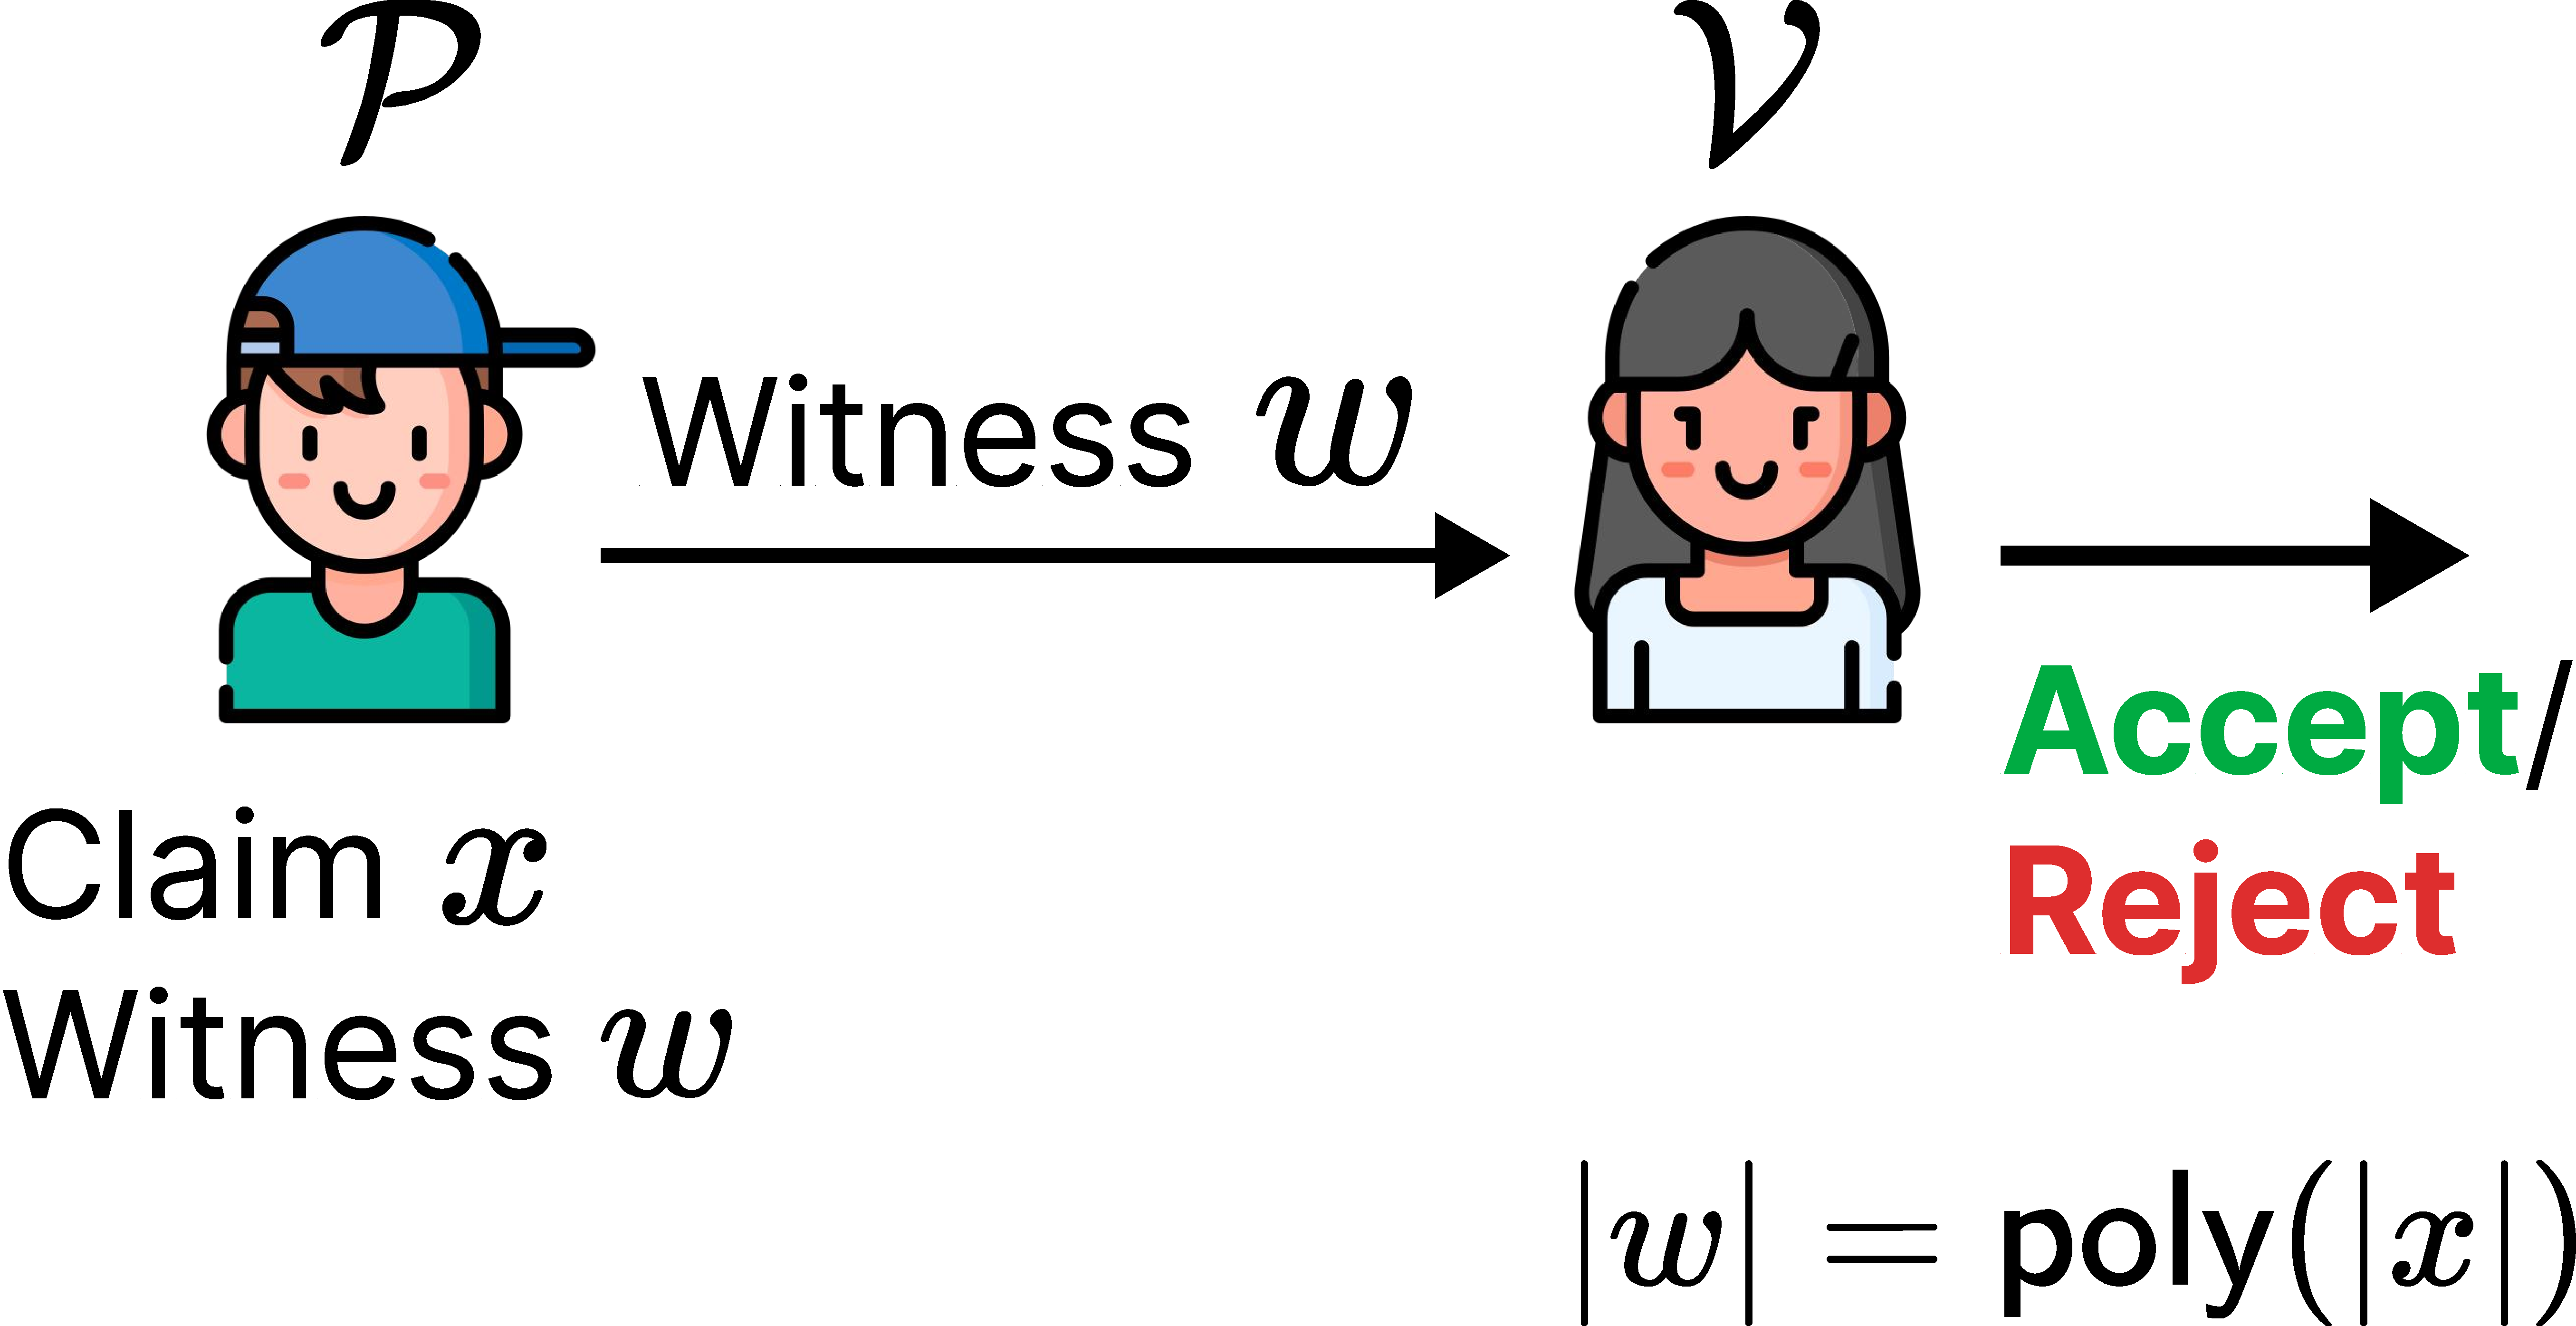
\includegraphics[width=0.7\textwidth]{images/lecture_6/np.pdf}
            \caption{Typical setup for cryptographic proofs.}
        \end{figure}
    \end{frame}

    \begin{frame}{NP Statements}
        \begin{definition}[P Language]
            Problem is in the $\mathbf{P}$ class if exists a polytime algorithm checking $x \in \mathcal{L}$.
        \end{definition}

        \begin{definition}[NP Language]
            A language $\mathcal{L}_{\mathcal{R}}$ belongs to the $\mathbf{NP}$ class if there exists a polynomial-time verifier $\mathcal{V}$ such that the following two properties hold:
            \begin{itemize}
                \item \textbf{Completeness:} If $x \in \mathcal{L}_{\mathcal{R}}$, then there is a witness $w$ such that $\mathcal{V}(x, w) = 1$ with $|w| = \mathsf{poly}(|x|)$. Essentially, it states that true claims have \textit{short} proofs.
                \item \textbf{Soundness:} If $x \not\in \mathcal{L}_{\mathcal{R}}$, then for any $w$ it holds that $\mathcal{V}(x, w) = 0$. Essentially, it states that false claims have no proofs.
            \end{itemize}
        \end{definition}

        \begin{theorem}
            Any $\mathbf{NP}$ problem has a zero-knowledge proof.
        \end{theorem}
    \end{frame}

    \begin{frame}{Question (aka Motivation)}
        But can we do better?

        Sending witness is\ldots Weird\ldots

        \begin{figure}
            \centering
            
\includegraphics[width=0.5\textwidth]{images/lecture_6/thonk.png}
            \caption{Hmm\ldots \#2}
        \end{figure}
    \end{frame}

    \section{Interactive Proofs}

    \subsection{Quadratic Residue Interactive Proof}
    \begin{frame}{Solution!}
        \begin{columns}
            % Description
            \begin{column}{0.4\textwidth}
                We add two more ingredients:
                \begin{itemize}
                    \item \textbf{Interaction:} instead of \textbf{passively} receiving the proof, the verifier $\mathcal{V}$ can \textbf{interact} with the prover $\mathcal{P}$ by sending \textbf{challenges} and receiving \textbf{responses}.
                    \item \textbf{Randomness:} $\mathcal{V}$ can send random coins (challenges) to the prover, which $\mathcal{P}$ can use to generate responses.
                \end{itemize}
            \end{column}
            \begin{column}{0.6\textwidth}
                \begin{figure}
                    \centering
                    \begin{tikzpicture}[scale=0.90, transform shape]
                        \node[inner sep=0pt, align=center] (prover) {
\includegraphics[width=1.25cm]{images/lecture_6/prover.png}\\Prover $\mathcal{P}$\\\textbf{Comp. Unbounded}};
                        \node[inner sep=0pt, align=center, right=1.5cm of prover] (verifier) {
\includegraphics[width=1.25cm]{images/lecture_6/verifier.png}\\Verifier $\mathcal{V}$ \\ \textbf{Probabilistic} \\ \textbf{Poly-Time (PPT)}};
                
                        \draw [dashed,line width=0.3mm] ([yshift=-0.5cm]prover.south) -- ([yshift=-5.0cm]prover.south);
                        \draw [dashed,line width=0.3mm] ([yshift=-0.5cm]verifier.south) -- ([yshift=-4.8cm]verifier.south);
                
                        \draw[-{Stealth[length=3mm]},line width=0.4mm] ([yshift=-1.5cm]prover.south) coordinate (l2)--(l2-|verifier) node[midway, above=0mm, fill=white]{Send $m_1$};
                
                        \draw[-{Stealth[length=3mm]},line width=0.4mm] ([yshift=-2.25cm]verifier.south) coordinate (l2)--(l2-|prover) node[midway, above=1mm, fill=white]{Toss coin $r_1$, send query $q_1$};
                
                        \draw[-{Stealth[length=3mm]},line width=0.4mm] ([yshift=-3.5cm]prover.south) coordinate (l2)--(l2-|verifier) node[midway, above=0mm, fill=white]{Send $m_2$};
                
                        \draw[-{Stealth[length=3mm]},line width=0.4mm] ([yshift=-4.25cm]verifier.south) coordinate (l2)--(l2-|prover) node[midway, above=1mm, fill=white]{Toss coin $r_2$, send query $q_2$};
                    \end{tikzpicture}
                \end{figure}
            \end{column}
        \end{columns}
    \end{frame}

    \begin{frame}{Quadratic Residue Interactive Proof}
        \begin{block}{Problem Statement}
            \begin{itemize}
                \item \textbf{Statement:} $x \in \mathcal{L}_{\mathcal{R}}$ where our \textbf{language} is defined as:
                \begin{equation*}
                    \mathcal{L}_{\mathcal{R}} = \{x \in \mathbb{Z}_N^{\times}: \exists w \in \mathbb{Z}_N^{\times} \; \text{such that} \; x \equiv w^2 \; (\text{mod}\, N)\}
                \end{equation*}
                \item \textbf{Witness:} $w = \text{modular square root of $x$}$.
            \end{itemize}
        \end{block}

        How does $\mathcal{P}$ and $\mathcal{V}$ interact? Consider the figure below.

        \begin{figure}
            \centering
            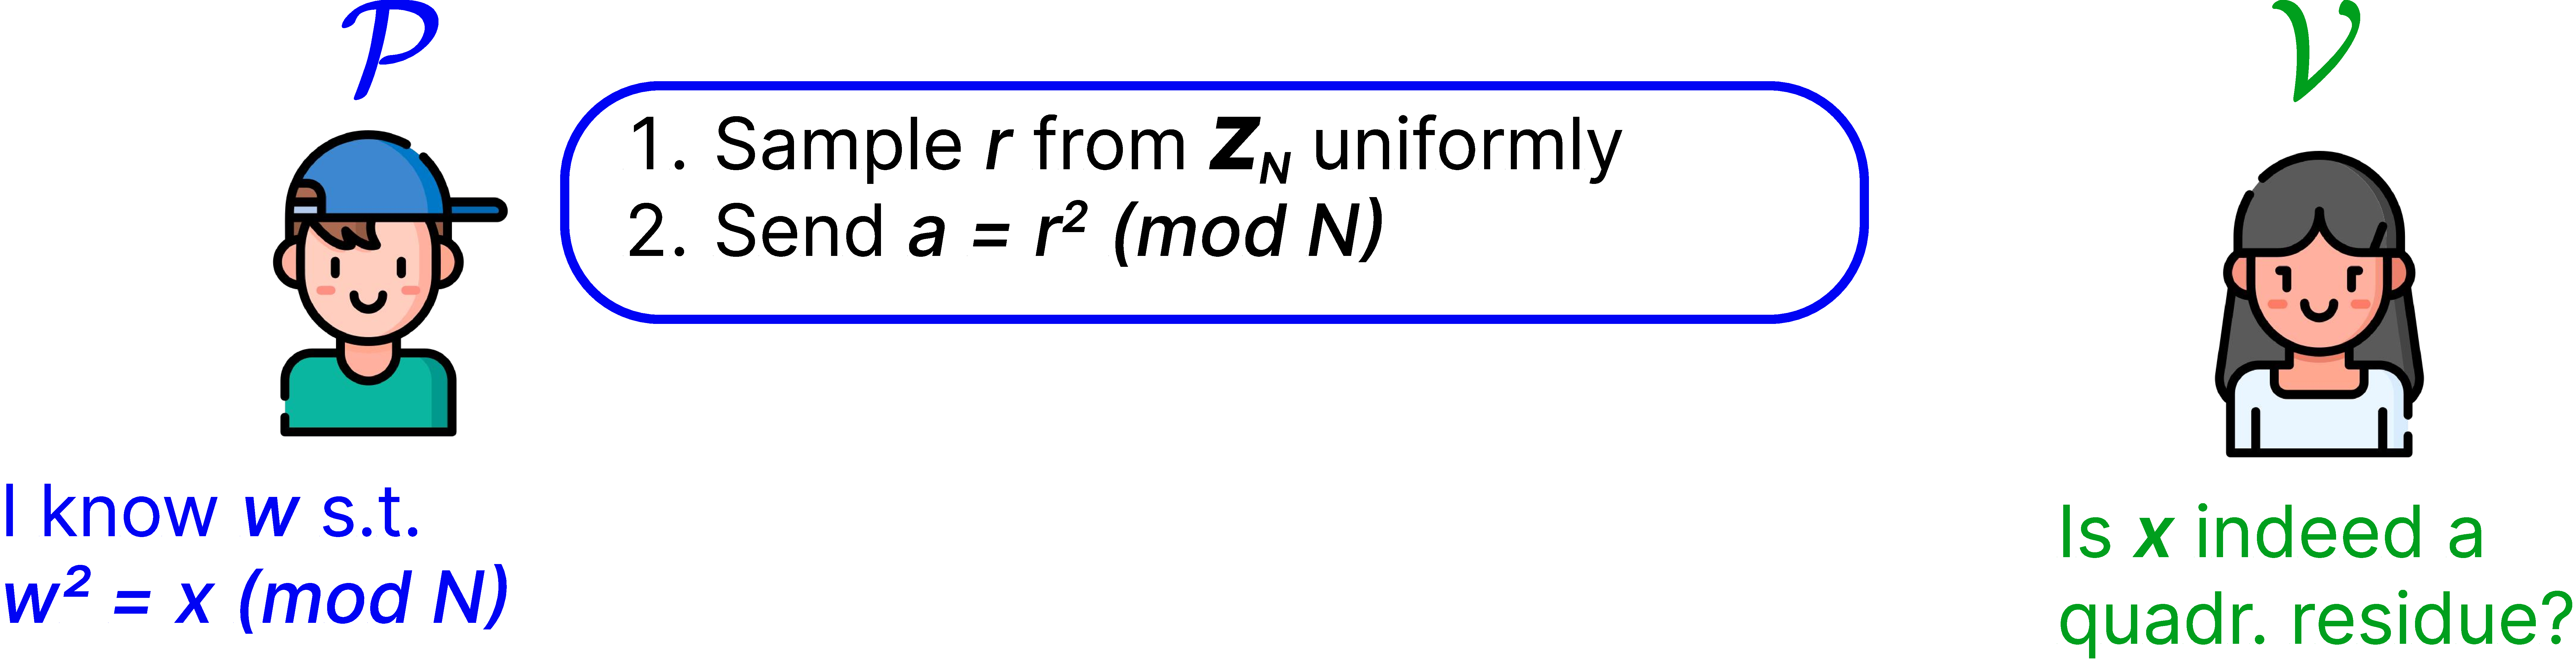
\includegraphics[width=\textwidth]{images/lecture_6/qr_test_1.pdf}
        \end{figure}
    \end{frame}

    \begin{frame}{Quadratic Residue Interactive Proof}
        \begin{figure}
            \centering
            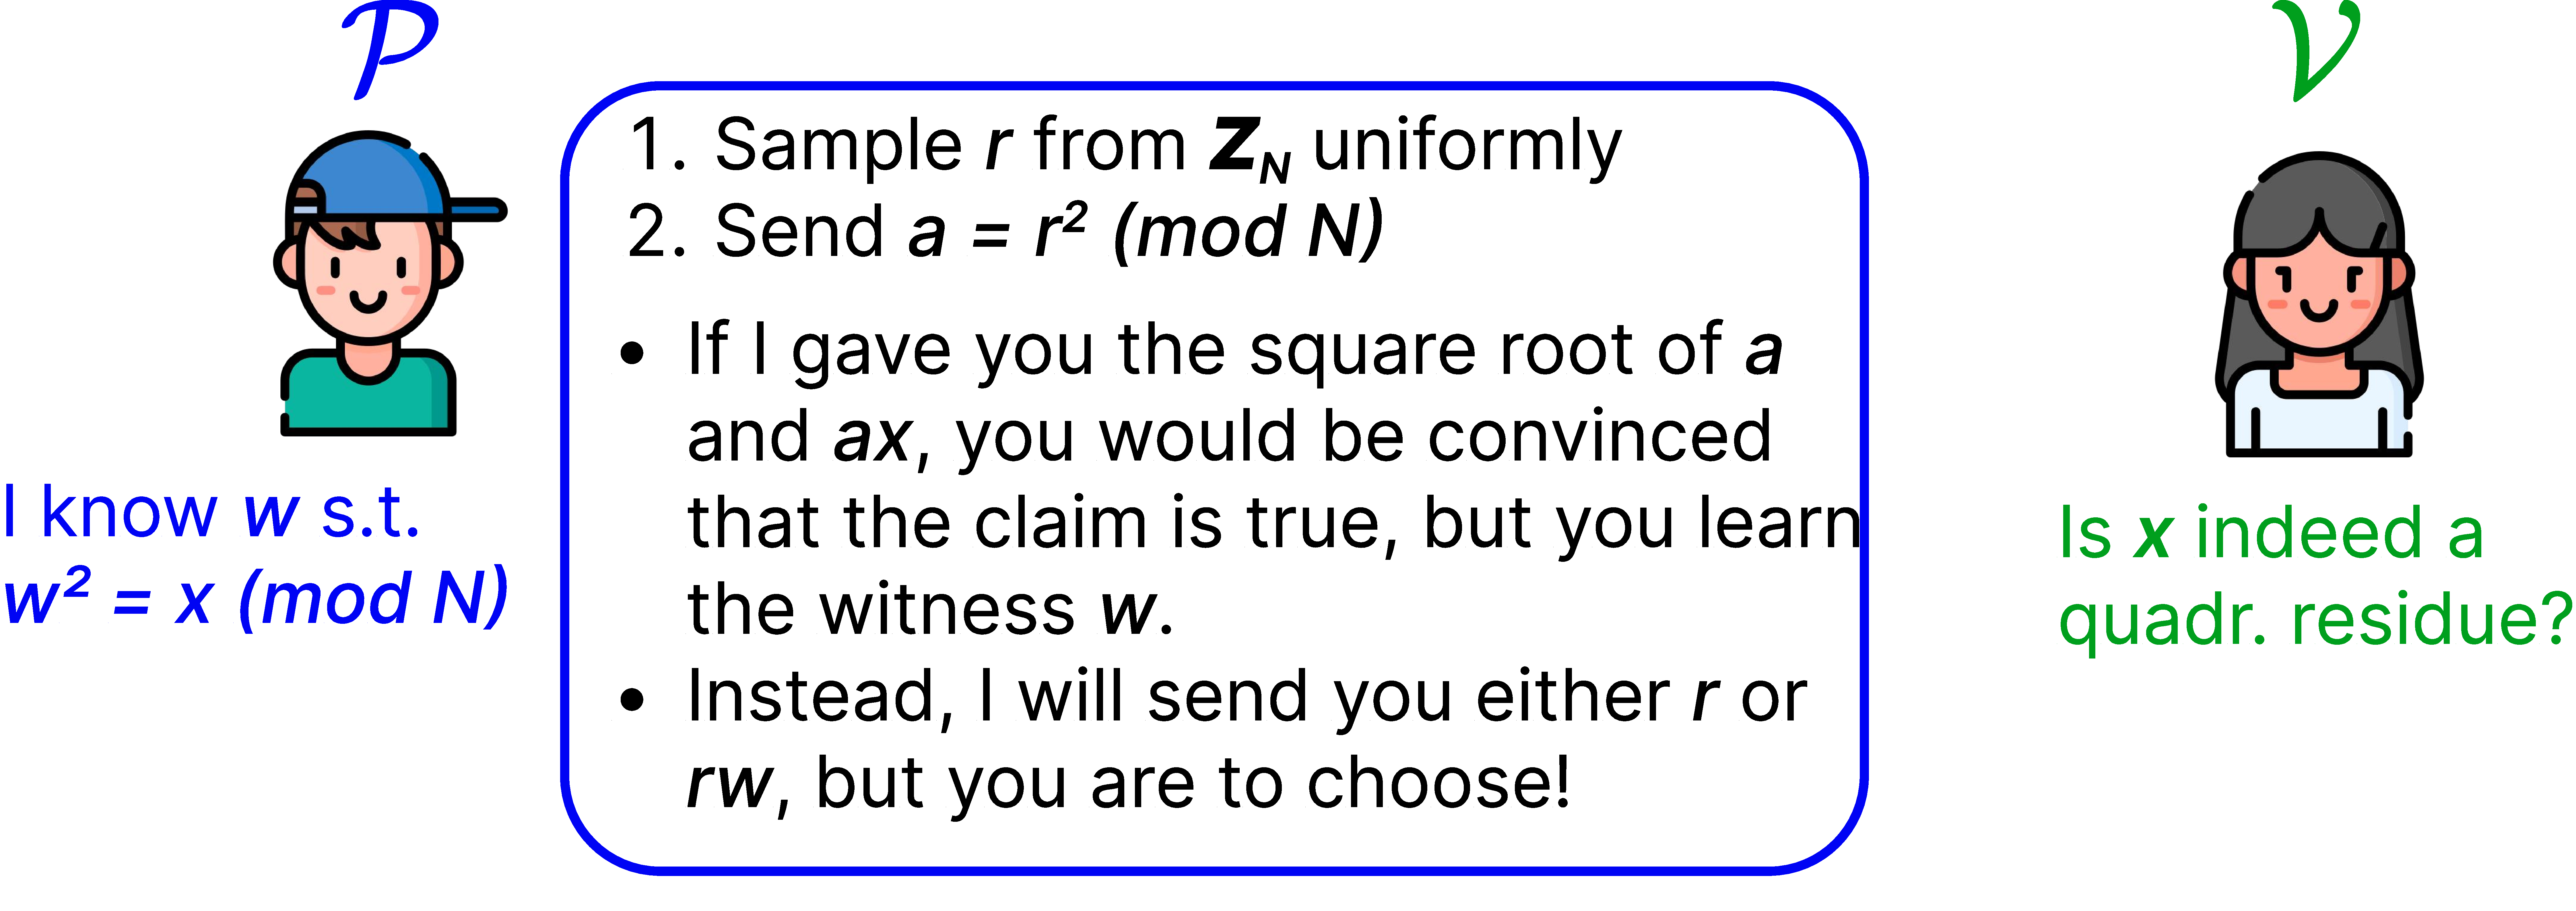
\includegraphics[width=\textwidth]{images/lecture_6/qr_test_2.pdf}
        \end{figure}
    \end{frame}

    \begin{frame}{Quadratic Residue Interactive Proof}
        \begin{figure}
            \centering
            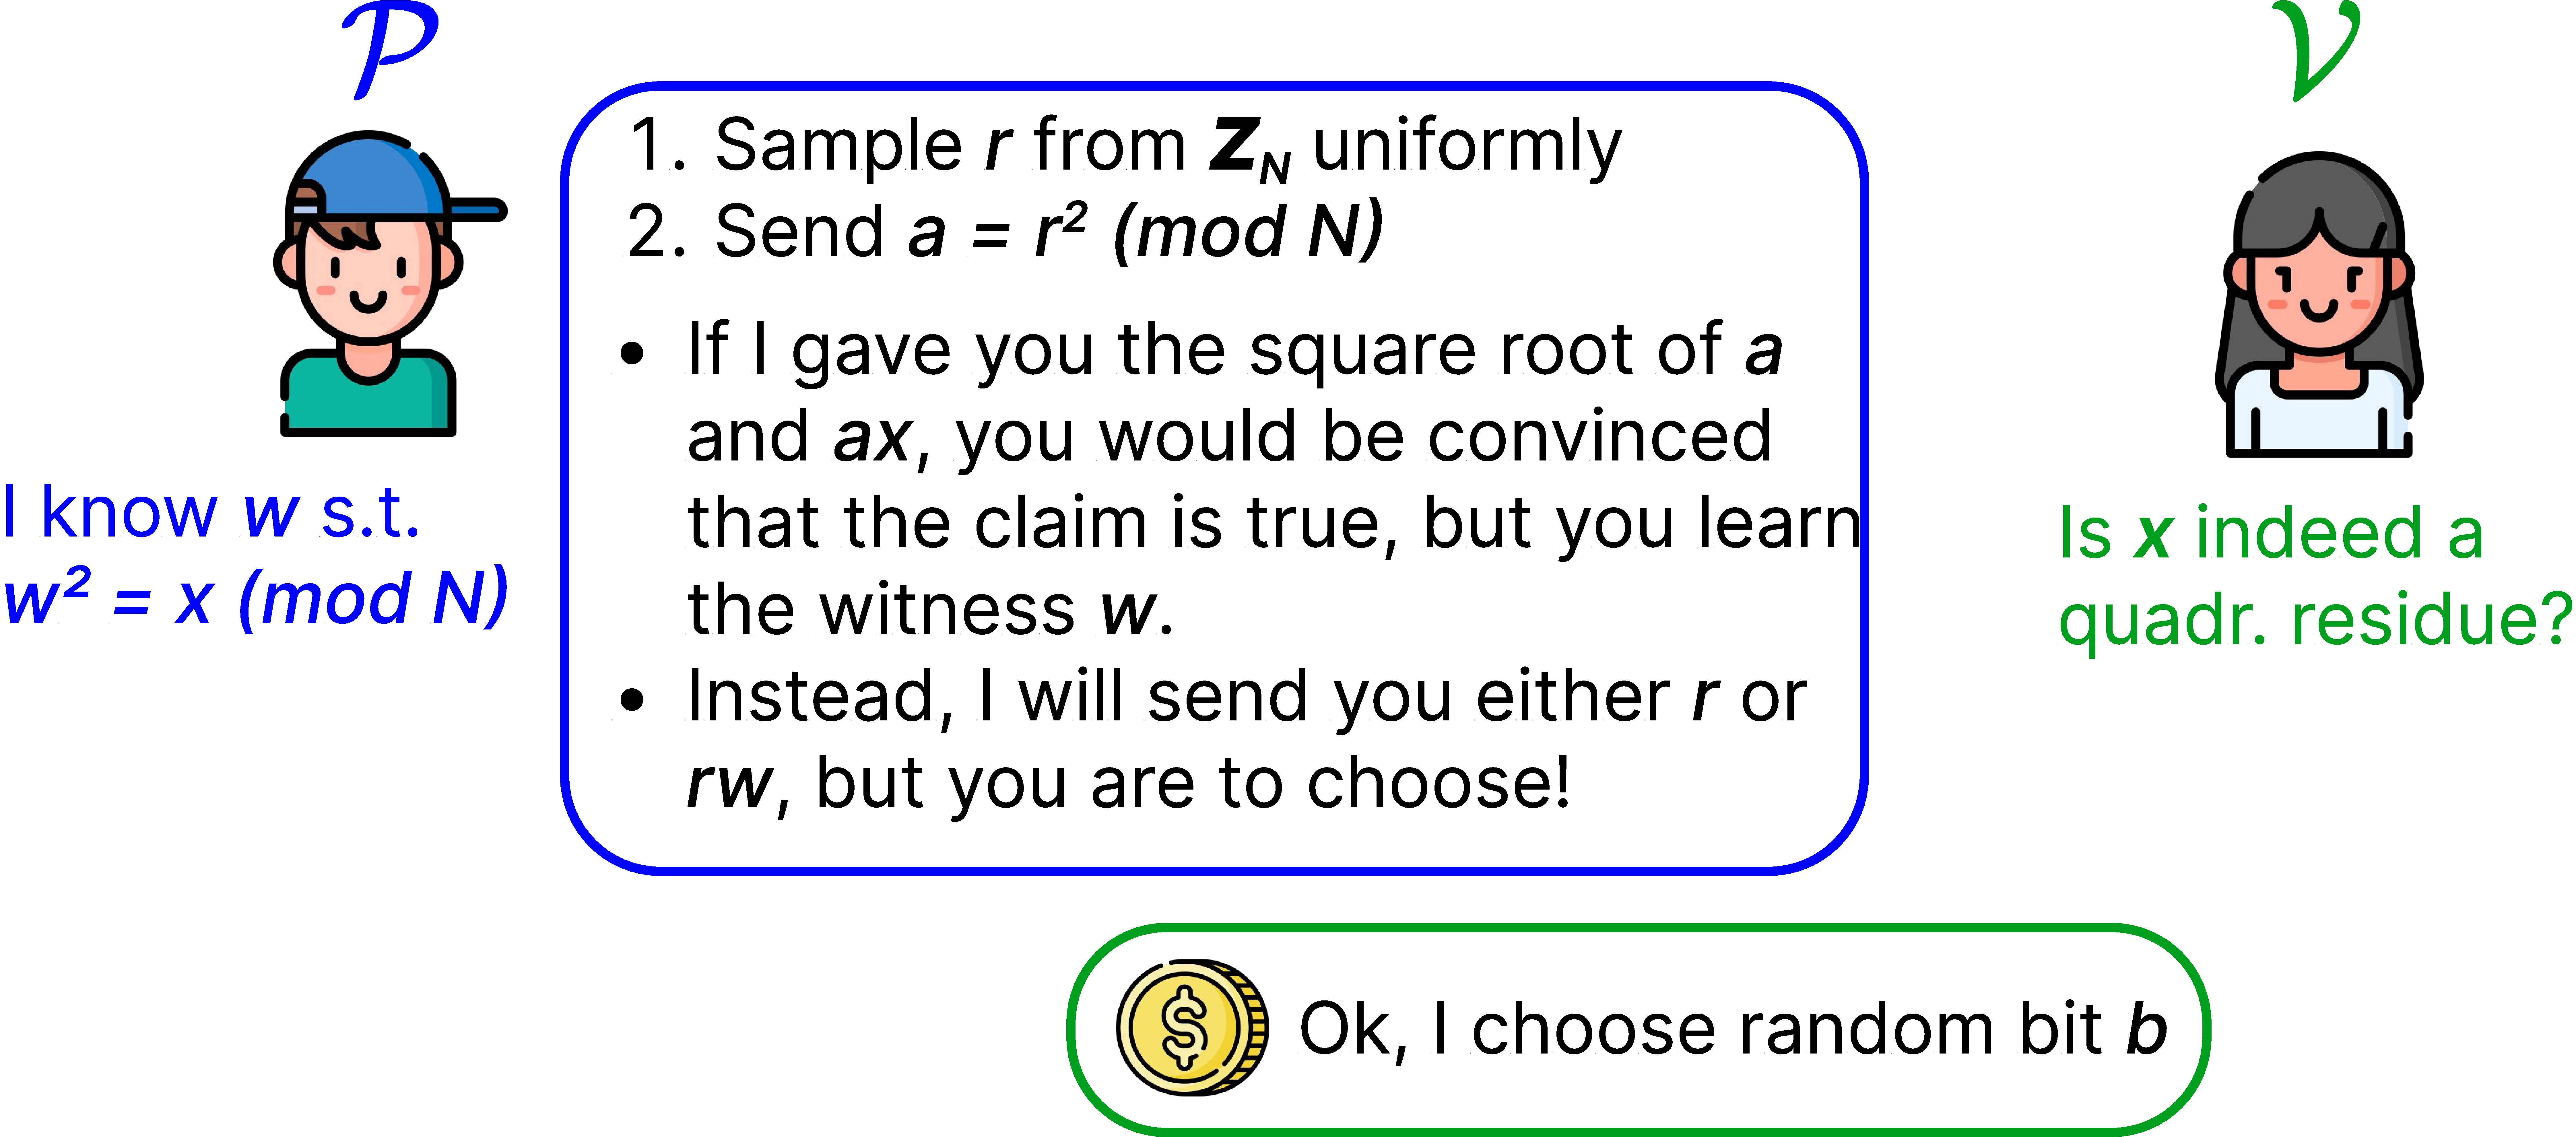
\includegraphics[width=\textwidth]{images/lecture_6/qr_test_3.pdf}
        \end{figure}
    \end{frame}

    \begin{frame}{Quadratic Residue Interactive Proof}
        \begin{figure}
            \centering
            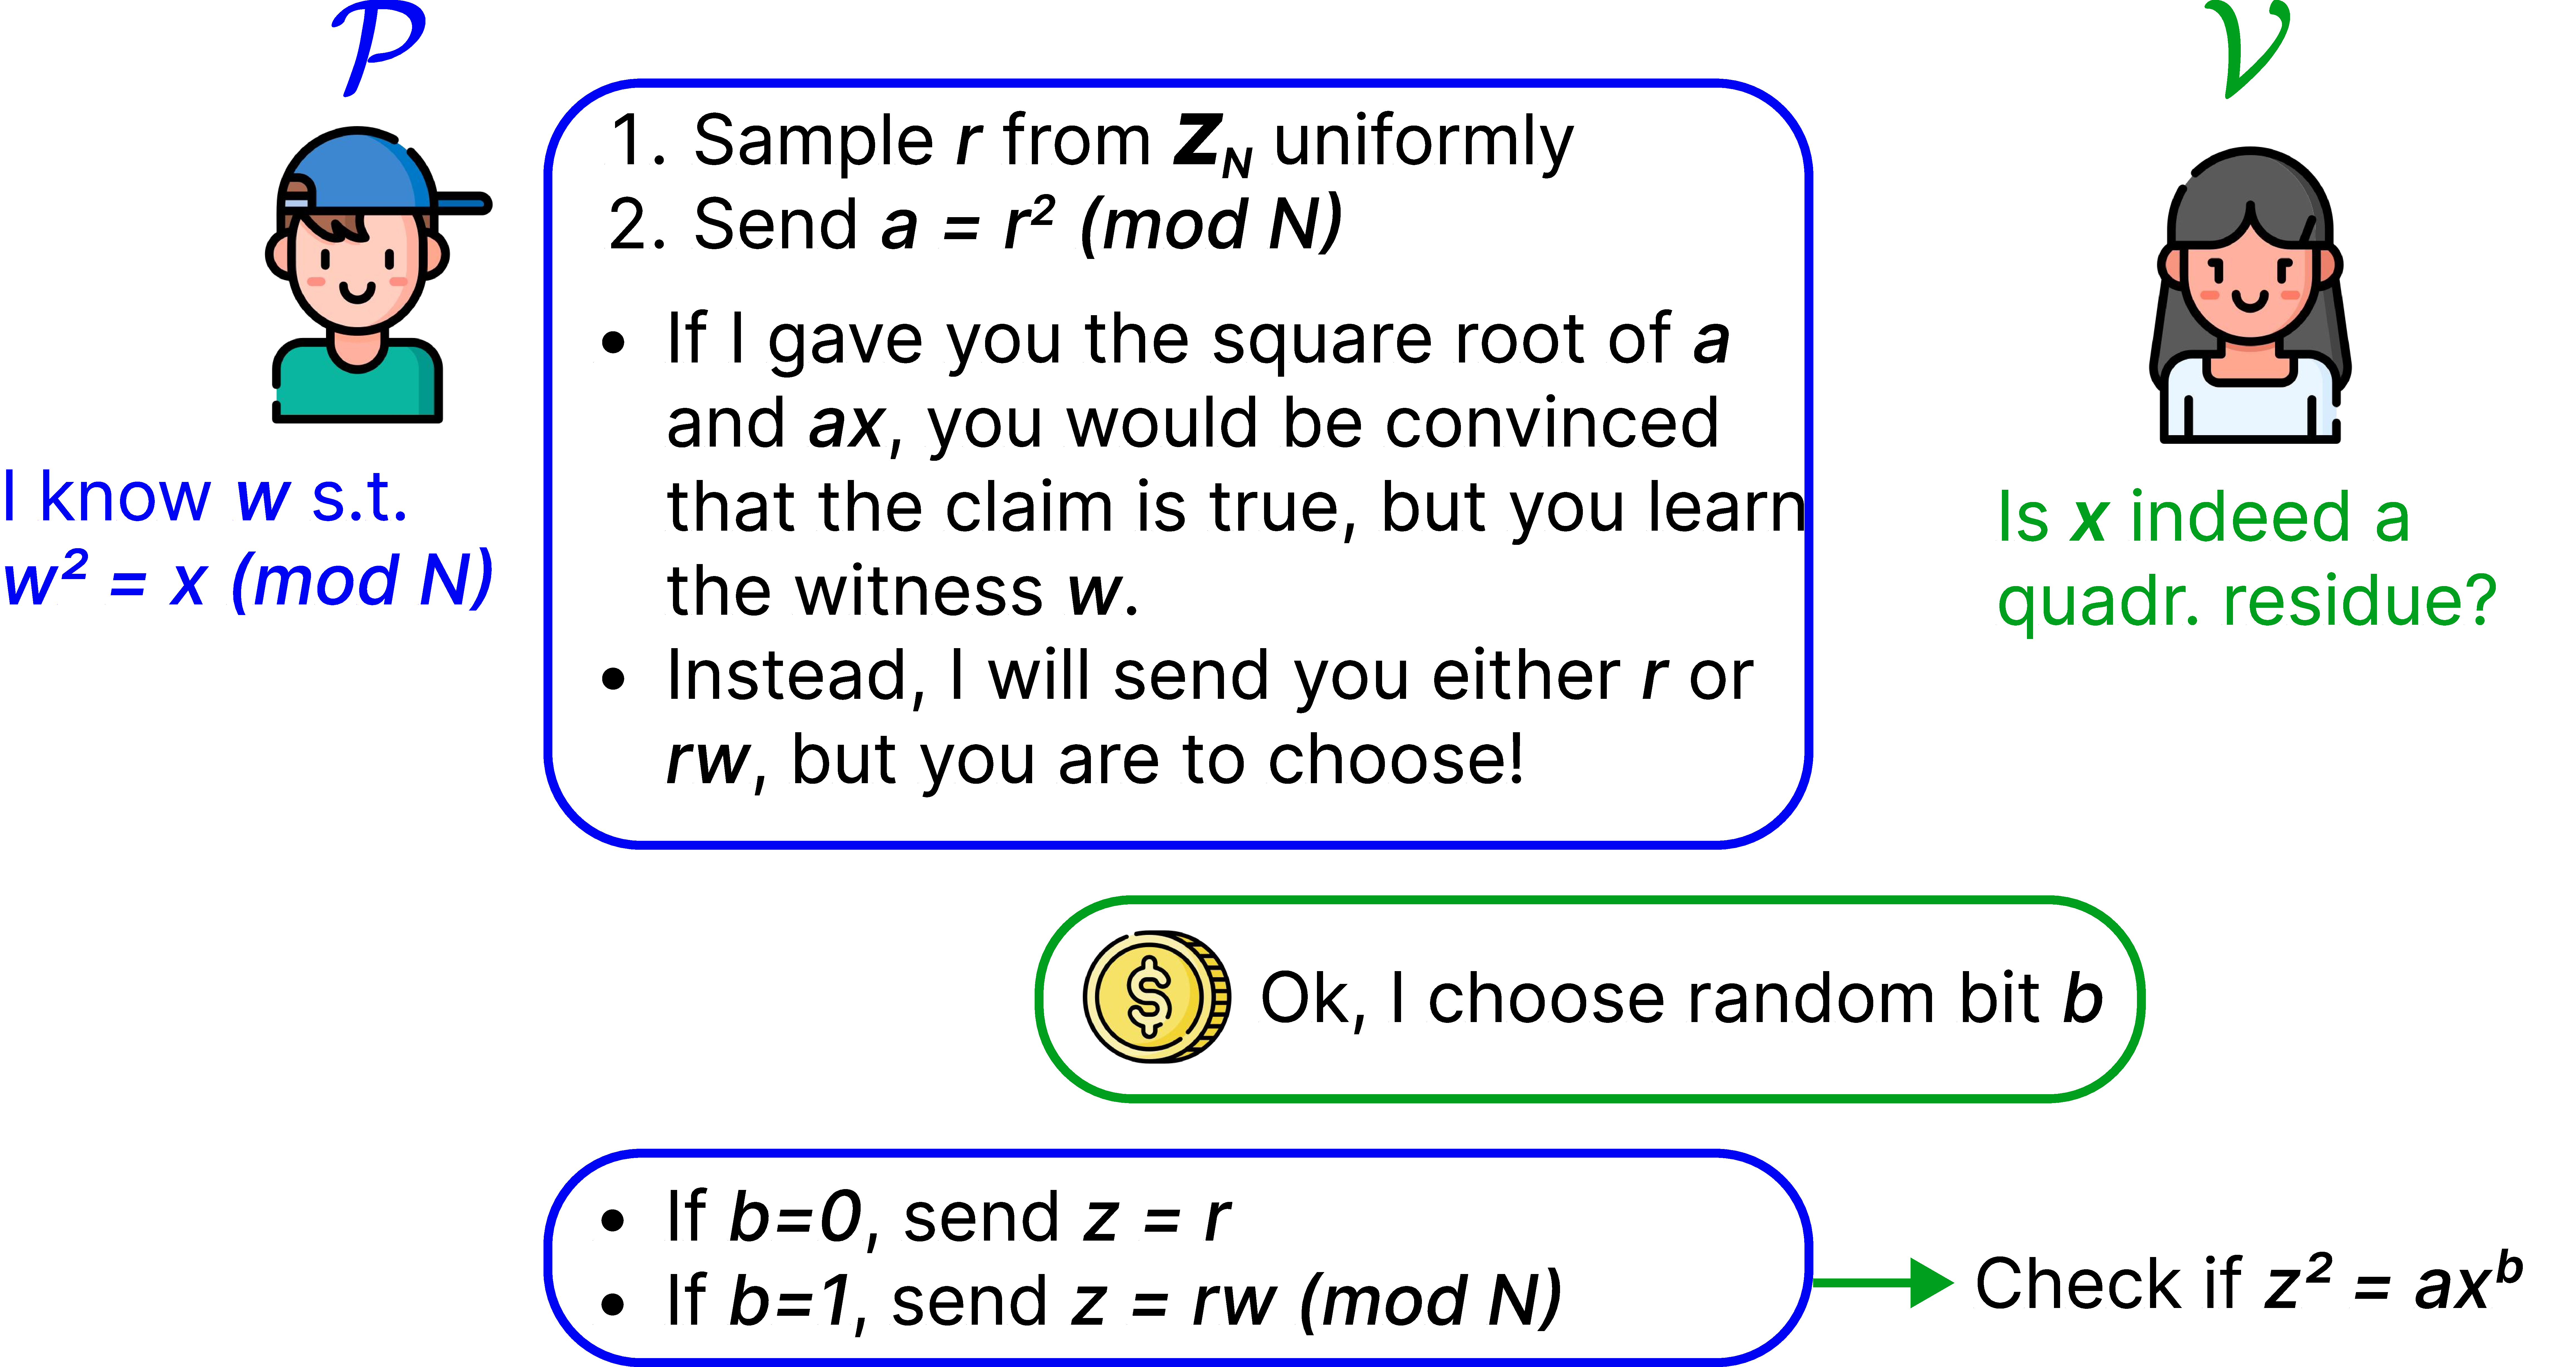
\includegraphics[width=\textwidth]{images/lecture_6/qr_test_4.pdf}
        \end{figure}
    \end{frame}

    \begin{frame}{Quadratic Residue Interactive Proof: Analysis}
        \begin{block}{Interactive Protocol}
            \begin{enumerate}
                \item $\mathcal{P}$ samples $r \xleftarrow{R} \mathbb{Z}_N^{\times}$ and sends $a = r^2$ to $\mathcal{V}$.
                \item $\mathcal{V}$ sends a random bit $b \in \{0,1\}$ to $\mathcal{P}$.
                \item $\mathcal{P}$ sends $z = r \cdot w^b$ to $\mathcal{V}$.
                \item $\mathcal{V}$ accepts if $z^2 = a \cdot x^b$, otherwise it rejects.
                \item Repeat $\lambda \in \mathbb{N}$ times.
            \end{enumerate}
        \end{block}

        \begin{lemma}
            The aforementioned protocol is \textbf{complete} and \textbf{sound}.
        \end{lemma}

        \textbf{Completeness.} If $b=0$, then $z=r$ and thus $z^2=r^2=a$, check passes.

        If $b=1$, then $z=rw$ and thus $z^2=r^2w^2=ax$, check passes.
    \end{frame}

    \subsection{Completeness and Soundness}
    \begin{frame}{Quadratic Residue Interactive Proof: Analysis}
        \textbf{Soundness.} The main reason why the protocol is sound is insribed in the theorem below.

        \begin{theorem}
            For any prover $\mathcal{P}^*$ with $x \not\in \mathcal{L}_{\mathcal{R}}$, the probability of $\mathcal{V}$ accepting the proof is at most $1/2$. 
        \end{theorem}

        \textbf{Corollary.} After repeating the protocol $\lambda$ times, we have
        \begin{equation*}
            \text{Pr}[\mathcal{V} \; \text{accepts after $\lambda$ rounds}] \leq \frac{1}{2^{\lambda}} = \mathsf{negl}(\lambda).
        \end{equation*}

        Thus, we showed both \textbf{completeness} and \textbf{soundness} of the protocol.
    \end{frame}

    \begin{frame}{Interactive Protocol Definition}
        \textcolor{gray}{$\langle \mathcal{P}, \mathcal{V} \rangle(x)$ reads as ``interaction between $\mathcal{P}$ and $\mathcal{V}$ on the statement $x$''.}

        \begin{definition}
            A pair of algorithms $(\mathcal{P},\mathcal{V})$ is called an \textbf{interactive proof} for a language $\mathcal{L}_{\mathcal{R}}$ if $\mathcal{V}$ is a polynomial-time verifier and the following two properties hold:
            \begin{itemize}
                \item \textbf{Completeness:} For any $x \in \mathcal{L}_{\mathcal{R}}$, $\text{Pr}[\langle \mathcal{P}, \mathcal{V} \rangle(x) = \mathsf{accept}]=1$.
                \item \textbf{Soundness:} For any $x \not\in \mathcal{L}_{\mathcal{R}}$ and for any prover $\mathcal{P}^*$, we have 
                \begin{equation*}
                    \text{Pr}[\langle \mathcal{P}^*, \mathcal{V} \rangle(x) = \mathsf{accept}] \leq \mathsf{negl}(\lambda)
                \end{equation*}
            \end{itemize}
        \end{definition}

        \begin{definition}
            \textbf{The class of interactive proofs} (\textbf{IP}) is defined as:
            \begin{equation*}
                \mathbf{IP} = \{\mathcal{L}: \text{there is an interactive proof $(\mathcal{P}, \mathcal{V})$ for $\mathcal{L}$}\}.
            \end{equation*}
        \end{definition}
    \end{frame}

    \subsection{Zero-Knowledge and Honest-Verifier Zero-Knowledge}
    \begin{frame}{Zero-Knowledge Informal Definition}
        \begin{definition}
            An interactive proof system $(\mathcal{P}, \mathcal{V})$ is called \textbf{zero-knowledge} if for any polynomial-time verifier $\mathcal{V}^*$ and any $x \in \mathcal{L}_{\mathcal{R}}$, the interaction $\langle \mathcal{P}, \mathcal{V}^* \rangle(x)$ gives nothing new about the witness $w$.
        \end{definition}
        
        \begin{definition}
            The pair of algorithms $(\mathcal{P}, \mathcal{V})$ is called a \textbf{zero-knowledge interactive protocol} if it is \textit{complete}, \textit{sound}, and \textit{zero-knowledge}.
        \end{definition}

        \begin{figure}
            \centering
            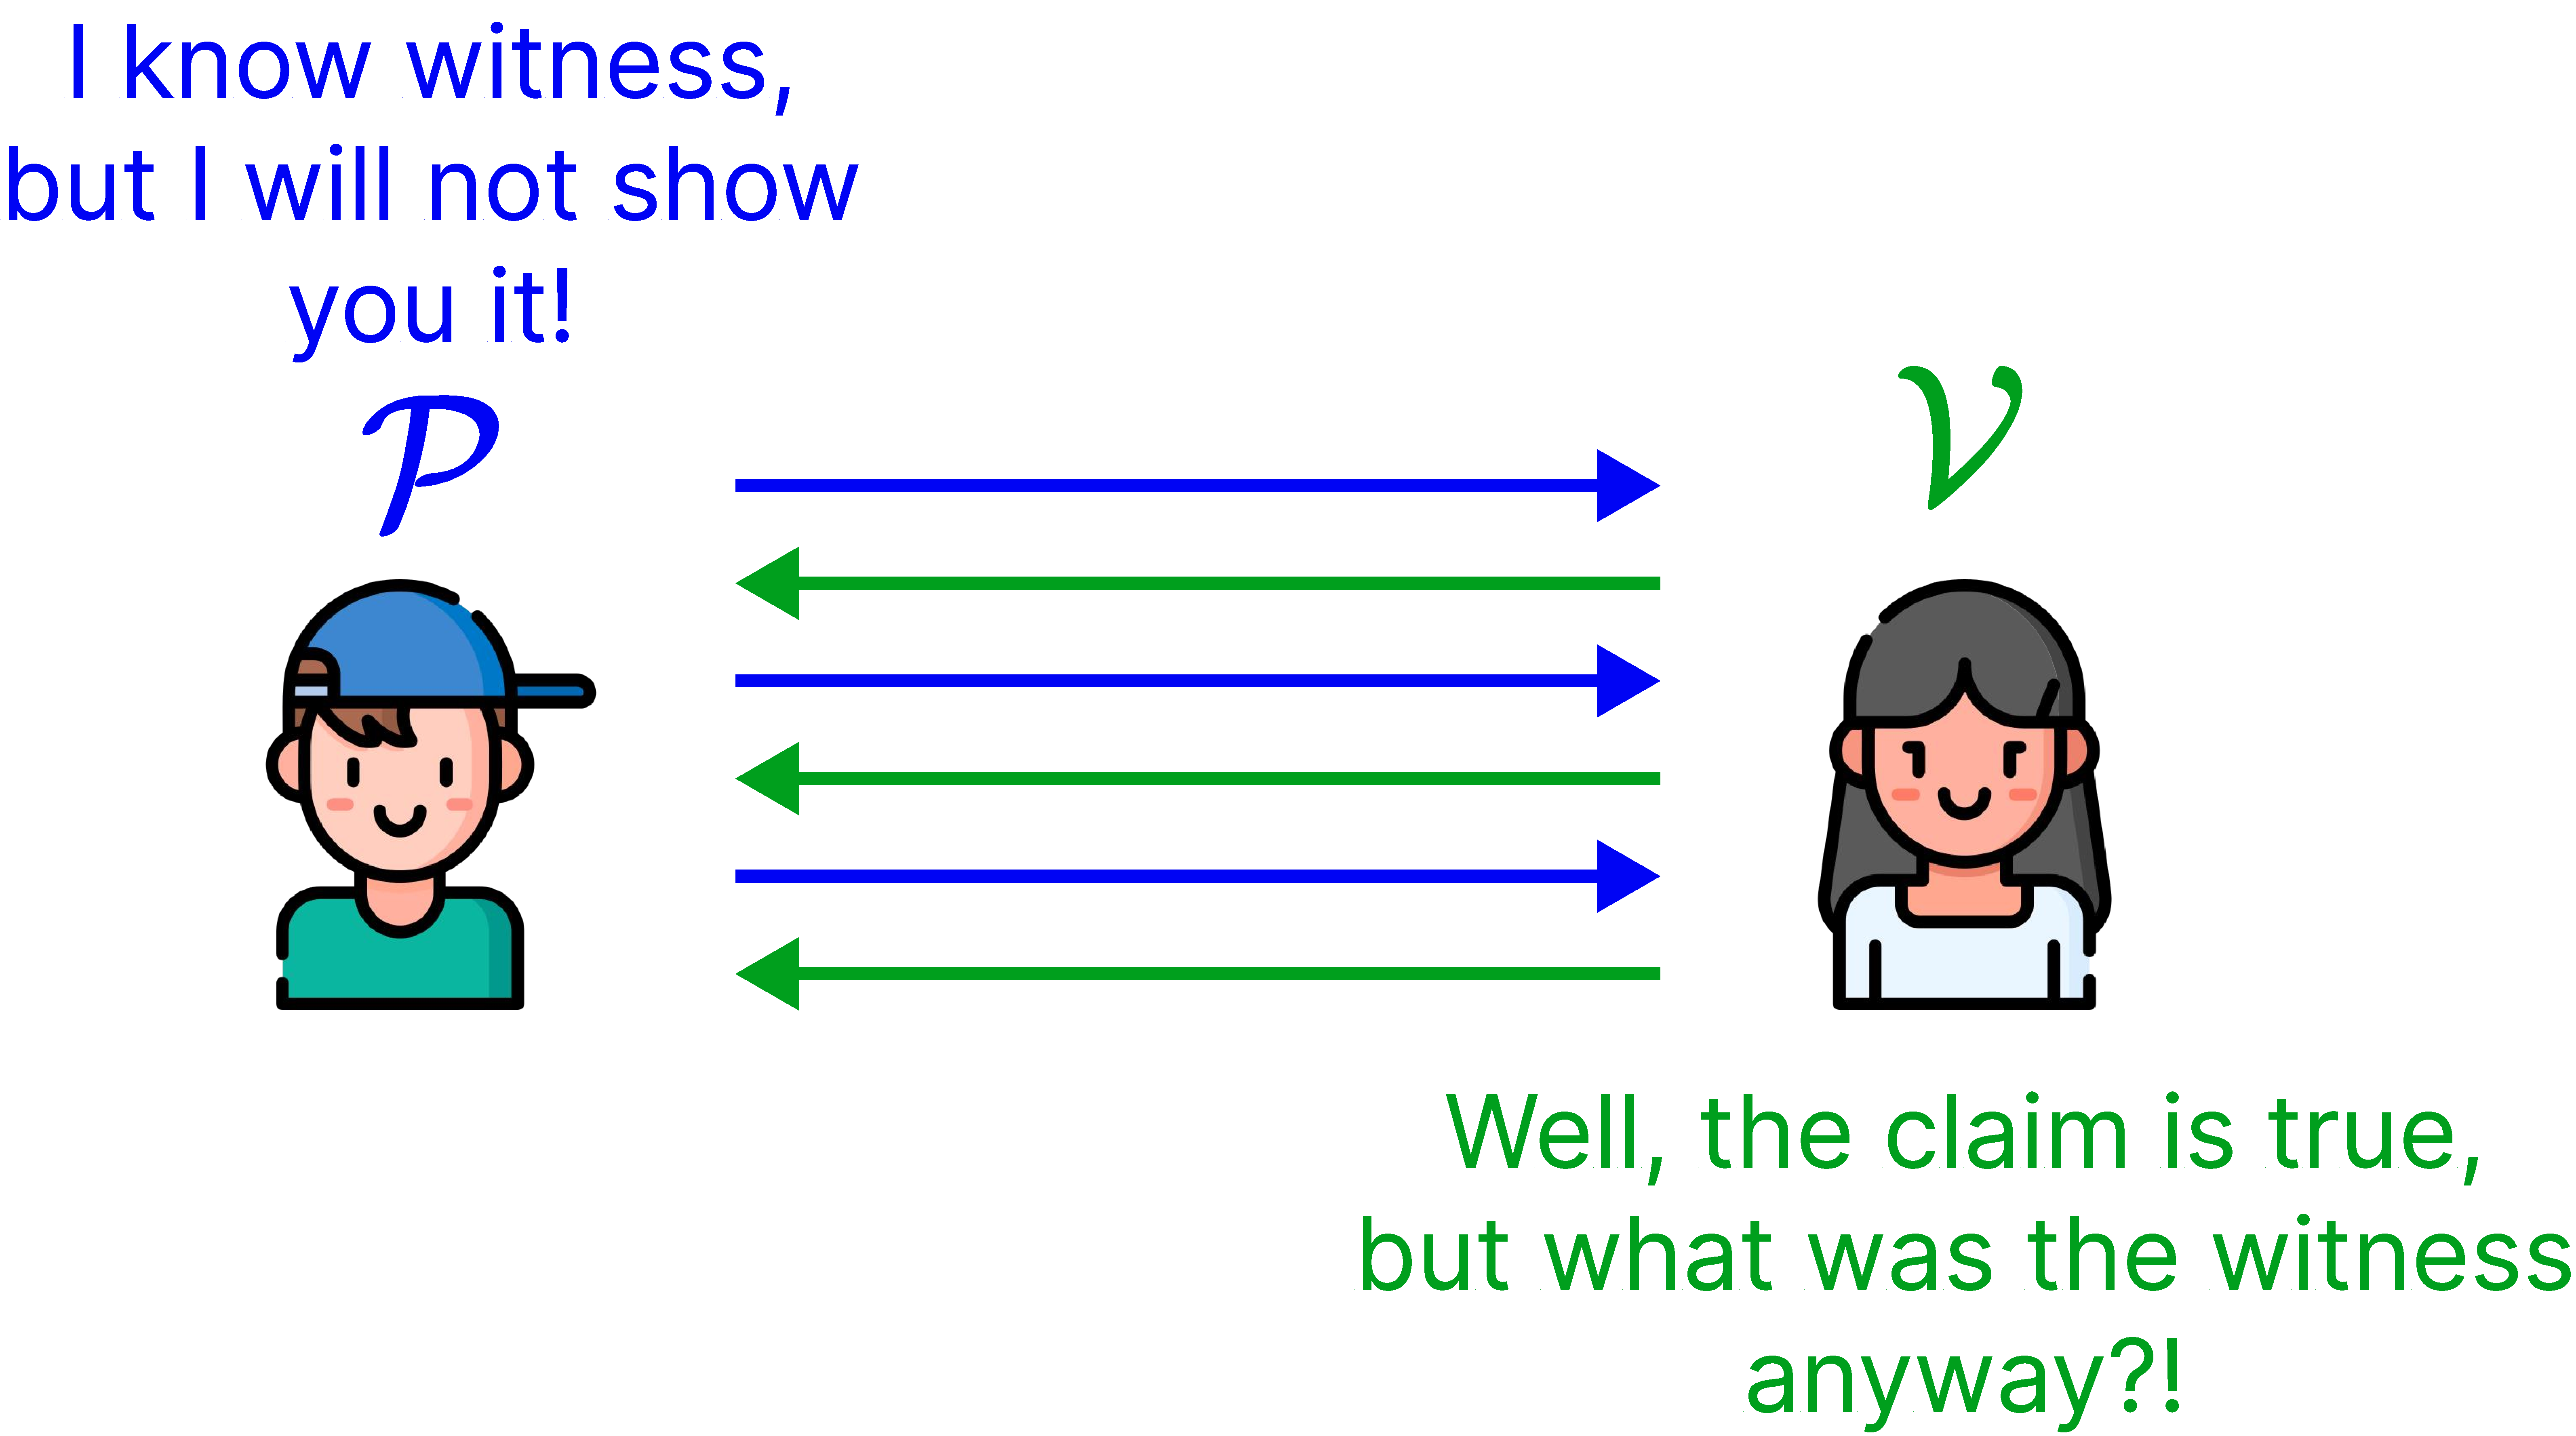
\includegraphics[width=0.5\textwidth]{images/lecture_6/zk.pdf}
        \end{figure}
    \end{frame}

    \begin{frame}{Verifier's View}
        \begin{alertblock}{Question \#1}
            What has the verifier learned during the interaction?
        \end{alertblock}

        \begin{itemize}
            \item First things first, he learned that the statement $x$ is true.
            \item He also knows queries $(q_1,\dots,q_{\ell})$ and random coins $(r_1,\dots,r_{\ell})$ he tossed (since he is the one who has sent them).
            \item Moreover, he knows the prover's messages $(m_1,m_2,\dots,m_{\ell})$.
        \end{itemize}

        \begin{definition}
            All the conversation that verifier has witnessed is called \textbf{verifier's view} and is denoted as
            \begin{equation*}
                \mathsf{view}_{\mathcal{V}}(\mathcal{P}, \mathcal{V}) = (m_1,r_1,q_1,m_2,r_2,q_2,\dots,m_{\ell},r_{\ell},q_{\ell}).
            \end{equation*} 
        \end{definition}

        \textcolor{purple}{\textbf{Fact:}} $\mathsf{view}_{\mathcal{V}}(\mathcal{P}, \mathcal{V})$ is a \textbf{random variable}.
    \end{frame}

    \begin{frame}{Verifier's View: Example}
        \begin{example}
            For QN test, set $N:=3 \times 2^{30} + 1$ (prime number), and $\mathcal{P}$ wants to convince that $1286091780 \in \mathcal{L}_R$. Conversation is the following:
            \begin{enumerate}
                \item During the first round, $\mathcal{P}$ sends $672192003$ to $\mathcal{V}$.
                \item $\mathcal{V}$ sends $b=0$ to $\mathcal{P}$.
                \item $\mathcal{P}$ sends $2606437826$ to $\mathcal{V}$.
                \item $\mathcal{V}$ verifies that indeed $2606437826^2 \equiv 672192003 \pmod{N}$.
                \item During the second round, $\mathcal{P}$ sends $2619047580$ to $\mathcal{V}$.
                \item $\mathcal{V}$ chooses $b=1$ and sends to $\mathcal{P}$.
                \item $\mathcal{P}$ sends $1768388249$ to $\mathcal{V}$.
                \item $\mathcal{V}$ verifies that $1768388249^2 \equiv 2619047580 \times 1286091780 \pmod{N}$.
                \item Conversation ends.
            \end{enumerate}
        \end{example}
    \end{frame}
            
    \begin{frame}{Verifier's View: Example}
        \begin{example}
            The \textbf{view of the verifier} $\mathcal{V}$ is the following: 
            \begin{align*}
                \mathsf{view}_{\mathcal{V}}(\mathcal{V}, \mathcal{P})[1286091780] \\= (672192003, 0, 2606437826, 2619047580, 1, 1768388249)
            \end{align*}
            
            \begin{itemize}
                \item Essentially, this view is the same as you have witnessed.
                \item You have not learned anything about $w$ that prover $\mathcal{P}$ knows.
                \item The witness was $w = 3042517305$ and two randomnesses were $r_1 = 2606437826$ and $r_2 = 3023142760$.
                \item This is a random variable: conversation could be different.
            \end{itemize}
        \end{example}
    \end{frame}

    \begin{frame}{Zero-Knowledge Formally: Simulation Paradigm}
        \begin{alertblock}{Question \#2}
            What does it mean that the protocol is zero-knowledge?
        \end{alertblock}

        \begin{itemize}
            \item Protocol is zero-knowledge if, given the verifier's $\mathsf{view}_{\mathcal{V}}(\mathcal{P}, \mathcal{V})$, verifier cannot infer any information about the witness $w$.
            \item What does it mean that verifier $\mathcal{V}$ learns nothing new? It means that this view could have been simulated by $\mathcal{V}$ \textit{without even running an interaction}.
            \item Call the view after the real interaction as \textbf{real view}, while the view after the simulation as \textbf{simulated view}.
        \end{itemize}

        \begin{block}{Note}
            Such idea of defining the zero-knowledge is called \textbf{simulation paradigm} and currently the most widely used way to prove zero-knowledge.
        \end{block}
    \end{frame}

    \begin{frame}{Computational Indistinguishability}
        \begin{figure}
            \centering
            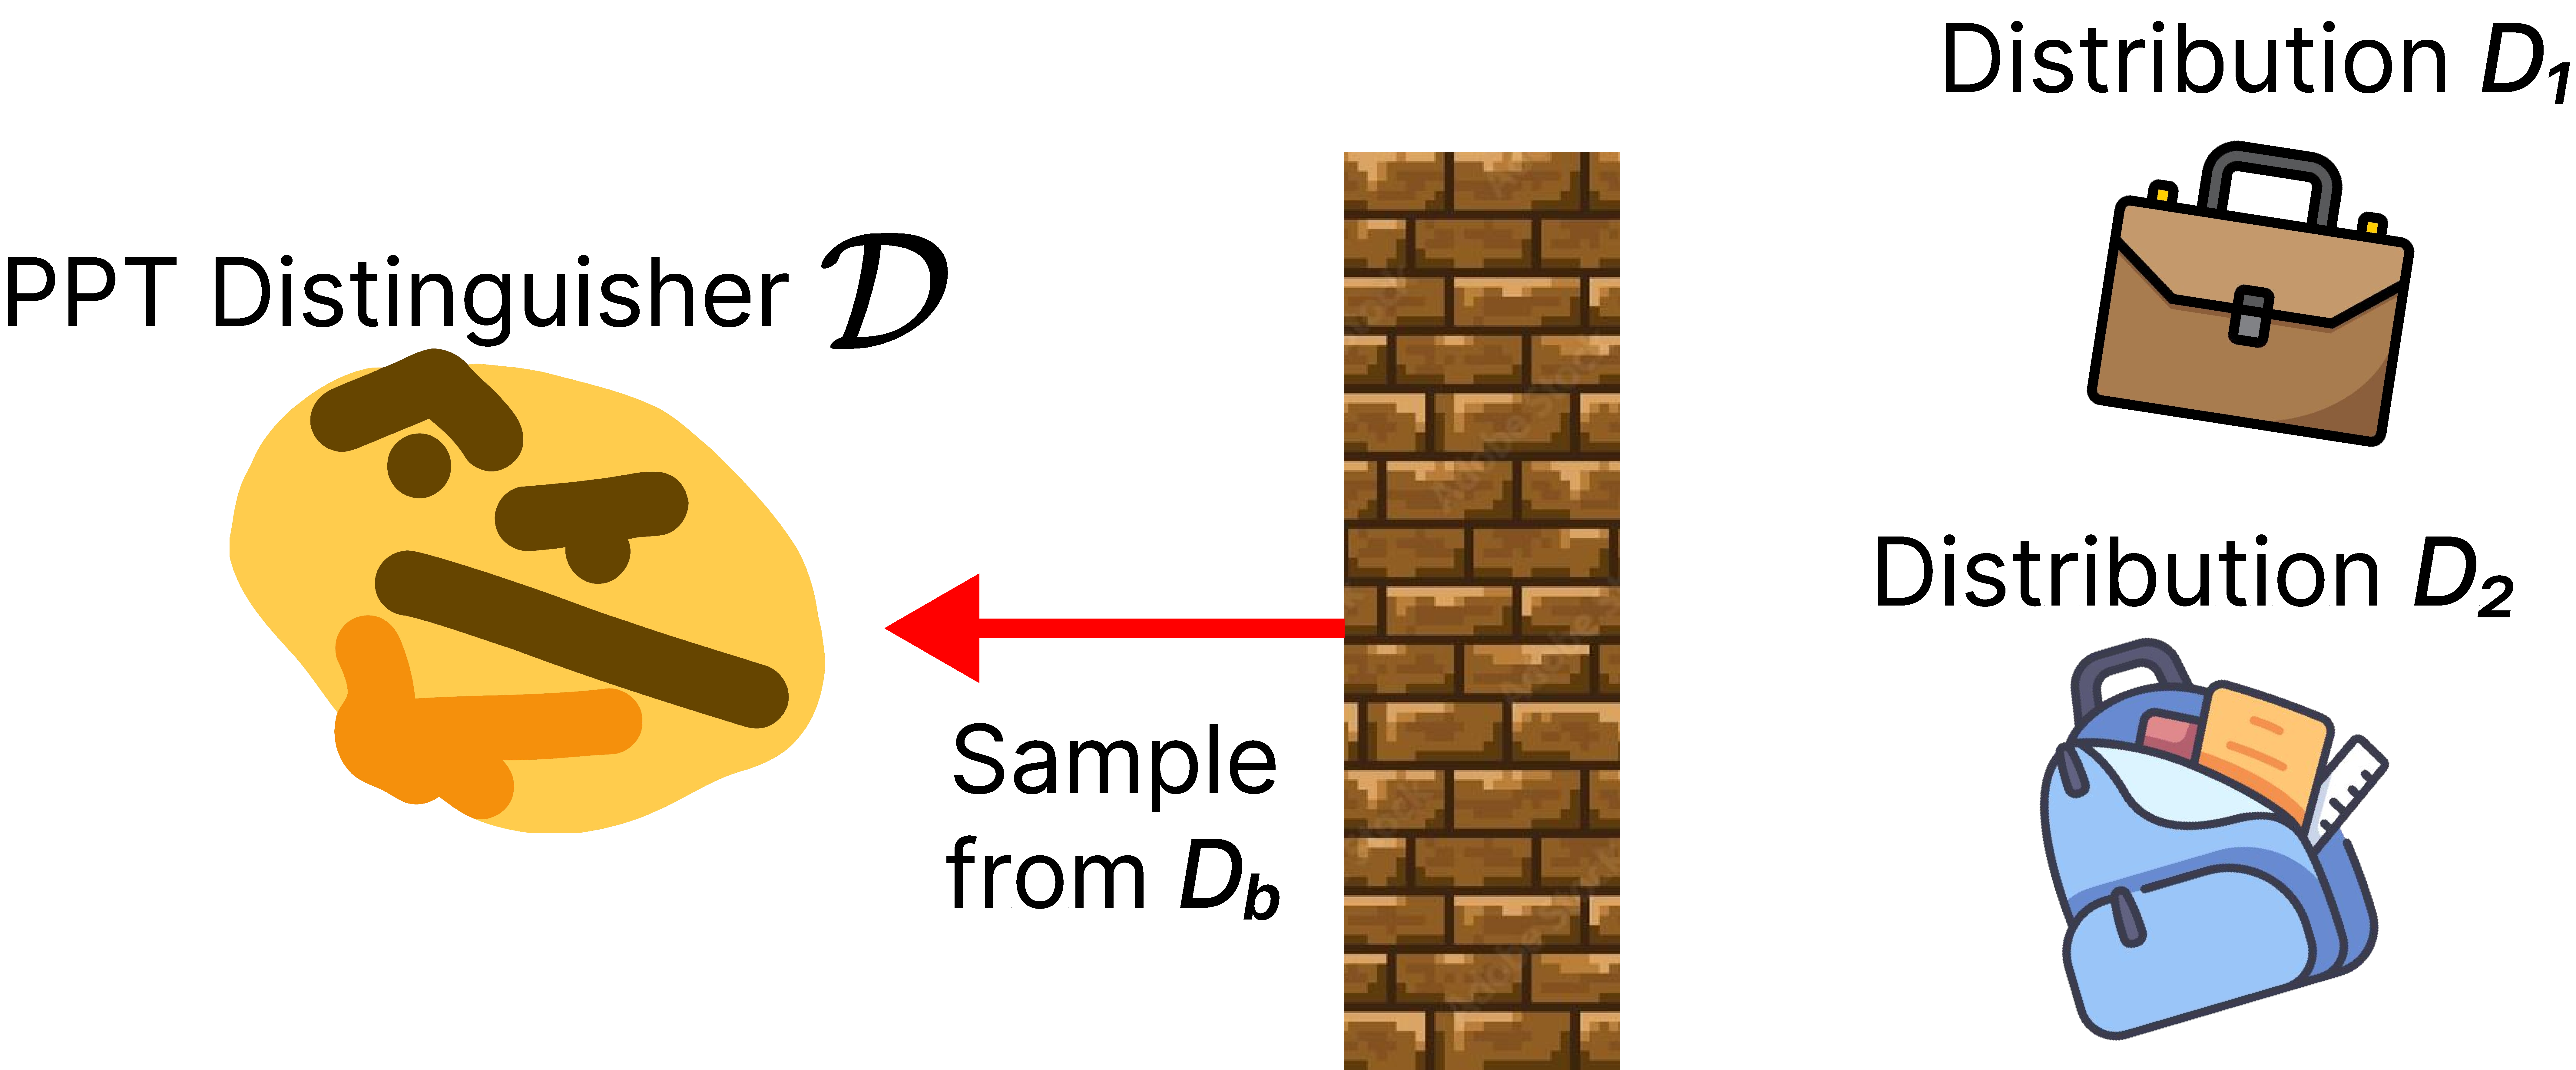
\includegraphics[width=0.8\textwidth]{images/lecture_6/cind.pdf}
        \end{figure}

        \begin{definition}[Informal Computational Indistinguisability]
            $D_1$ and $D_2$ are \textbf{computationally indistinguishable} (denoted by $D_1 \approx D_2$) if for any PPT distinguisher $\mathcal{D}$, even after polynomial number $k$ of samples from $D_b$ (where $b \xleftarrow{R} \{0,1\}$), for prediction $\hat{b}$: $\text{Pr}[\hat{b} = b] < \frac{1}{2} + \mathsf{negl}(k)$.
        \end{definition}
    \end{frame}

    \begin{frame}{Zero-Knowledge Formally (Kind of)}
        Finally, we are ready to define the \textbf{zero-knowledge}.

        \begin{definition}[Honest-Verifier Zero-Knowledge (HVZK)]
            An interactive protocol $(\mathcal{P}, \mathcal{V})$ is \textbf{honest-verifier zero-knowledge (HVZK)} for a language $\mathcal{L}_{\mathcal{R}}$ there exists a poly-time simulator $\mathsf{Sim}$ such that for any valid statement $x \in \mathcal{L}_{\mathcal{R}}$:
            \begin{equation*}
                \mathsf{view}_{\mathcal{V}}(\mathcal{P}, \mathcal{V})[x] \approx \mathsf{Sim}(x, \textcolor{gray}{1^{\lambda}})
            \end{equation*}
        \end{definition}

        \begin{definition}[Zero-Knowledge (ZK)]
            An interactive protocol $(\mathcal{P}, \mathcal{V})$ is \textbf{zero-knowledge (ZK)} for a language $\mathcal{L}_{\mathcal{R}}$ if \textit{for every poly-time verifier} $\mathcal{V}^*$ there \textit{exists a poly-time simulator} $\mathsf{Sim}$ such that for any valid statement $x \in \mathcal{L}_{\mathcal{R}}$:
            \begin{equation*}
                \mathsf{view}_{\mathcal{V}^*}(\mathcal{P}, \mathcal{V}^*)[x] \approx \mathsf{Sim}(x, \textcolor{gray}{1^{\lambda}})
            \end{equation*}
        \end{definition}
    \end{frame}

    \subsection{Proof of Knowledge}

    \begin{frame}{Proof of Knowledge: Why?}
        Now, the main issue with the above definition is that \textit{we have proven the statement correctness, but we have not proven that the prover \textbf{knows} the witness}. These are completely two distinct things!

        \begin{example}
            Consider the \textbf{discrete logarithm relation and language} for a cyclic group $E(\mathbb{F}_p)$ of order $r$:
            \begin{align*}
                \mathcal{R} = \{(P, \alpha) \in E(\mathbb{F}_p) \times \mathbb{Z}_r: P = [\alpha] G\}, \\ \mathcal{L}_{\mathcal{R}} = \{P \in E(\mathbb{F}_p): \exists \alpha \in \mathbb{Z}_r \; \text{such that} \; P = [\alpha] G\}
            \end{align*}
        \end{example}

        \begin{alertblock}{Question}
            What does it mean that $X \in \mathcal{L}_{\mathcal{R}}$?
        \end{alertblock}

        Turns out $\mathcal{L}_{\mathcal{R}} = E(\mathbb{F}_p)$, so the proof $X \in \mathcal{L}_{\mathcal{R}}$ itself is useless.
    \end{frame}

    \begin{frame}{Proof of Knowledge: Definition}
        \begin{enumerate}
            \item The knowledge of witness means that we can \textbf{extract} the witness while interacting with the prover.
            \item Thus, there should be an algorithm called \textbf{extractor} $\mathcal{E}$ which can extract the witness $w$.
            \item $\mathcal{E}$ is given more power than $\mathcal{V}$ (otherwise, if the protocol is zero-knowledge, we cannot extract $w$). $\mathcal{E}$ can \textbf{rewind} and \textbf{call} prover $\mathcal{P}$ multiple times.
            \item Sometimes, this is referred to as ``extractor $\mathcal{E}$ uses $\mathcal{P}$ as an oracle''.
        \end{enumerate}

        \begin{definition}[Proof of Knowledge]
            The interactive protocol $(\mathcal{P}, \mathcal{V})$ is a \textbf{proof of knowledge} for $\mathcal{L}_{\mathcal{R}}$ if exists a poly-time extractor algorithm $\mathcal{E}$ such that for any valid statement $x \in \mathcal{L}_{\mathcal{R}}$, in expected poly-time $\mathcal{E}^{\mathcal{P}}(x)$ outputs $w$ such that $(x,w) \in \mathcal{R}$.
        \end{definition}
    \end{frame}

    \begin{frame}{Proof of Knowledge: Example}
        \begin{lemma}
            The quadratic residue interactive protocol is a proof of knowledge.
        \end{lemma}
        
        \textbf{Proof.} Let us define the extractor $\mathcal{E}$ for the statement $x$ as follows:
        \begin{enumerate}
            \item Run the prover to receive $a \equiv r^2 \pmod{N}$ ($r$ is chosen randomly from $\mathbb{Z}_N^*$).
            \item Set verifier's message to $b=0$ to get $z_1 \gets r$.
            \item \textbf{Rewind} and set verifier's message to $b=1$ to get $z_2 \gets rw \pmod{N}$.
            \item Output $z_2/z_1 \pmod{N}$
        \end{enumerate}
        
        The extractor $\mathcal{E}$ will always output $w$ if $x \in \mathcal{L}_{\mathcal{R}}$. $\hfill\Box$
    \end{frame}

    \section{Fiat-Shamir Heuristic}
    \subsection{Cryptographic Oracles}
    \begin{frame}{Cryptographic Oracle}
        \begin{definition}[Cryptographic Oracle]
            Informally, \textit{cryptographic oracle} is simply a function $\mathcal{O}$ that gives in $O(1)$ an answer to some typically very hard problem.     
        \end{definition}
        
        \begin{example}[CDH Problem]
            Consider the \textbf{Computational Diffie-Hellman (CDH)} problem on the cyclic elliptic curve $E(\mathbb{F}_p)$ of prime order $r$ with a generator $G$. 
            
            \textbf{Hard Problem:} $[\alpha\beta]G$ given $[\alpha]G$ and $[\beta]G$ where $\alpha,\beta \in \mathbb{Z}_r$. 
        
            \textbf{Oracle:} However, we \textit{could} assume that such problem can be solved in $O(1)$ by a cryptographic oracle $\mathcal{O}_{\text{CDH}}: ([\alpha]G,[\beta]G) \mapsto [\alpha\beta]G$. 
            
            This way, we can rigorously prove the security of some cryptographic protocols \textit{even} if the Diffie-Hellman problem is suddenly solved. 
        \end{example}
    \end{frame}

    \begin{frame}{Random Oracle (RO)}
        One of the most popular cryptographic oracles is the \textbf{random oracle} $\mathcal{O}_{\text{R}}$. 

        \begin{definition}[Informal definition of RO]
            Suppose someone is inputting $x$ to the random oracle $\mathcal{O}_{\text{R}}: \mathcal{X} \to \mathcal{Y}$\footnote{Typically, RO works with a family of functions $f: \mathcal{X} \to \mathcal{Y}$, but we are not going too deep into the details.}. The oracle $\mathcal{O}_{\text{R}}$ does the following:
            \begin{enumerate}
                \item If $x$ has been queried before, the oracle returns the same value as it returned before.
                \item If $x$ has not been queried before, the oracle returns a randomly uniformly sampled value from the output space $\mathcal{Y}$.
            \end{enumerate}
        \end{definition}

        \begin{alertblock}{Question}
            Which very well-known cryptographic object can ``serve'' as a random oracle?
        \end{alertblock}
    \end{frame}
    \subsection{Fiat-Shamir Transformation}
    \begin{frame}{Fiat-Shamir Transformation}
        \begin{block}{Statement}
            \textbf{Any} interactive public-coin protocol can be converted into a non-interactive public-coin protocol with preserving completeness, soundness, and zero-knowledge using the random oracle.
        \end{block}

        One of such transformations is called \textbf{Fiat-Shamir heuristic}. Idea:
        \begin{enumerate}
            \item If all what $\mathcal{V}$ does is sending uniformly random values, this is an overkill.
            \item Instead of $\mathcal{V}$ sending random values, prover should be able to generate it himself, but he should not know the randomness in advance.
            \item Thus, we can replace the verifier's messages with the hash (random oracle) of all the previous conversation.
        \end{enumerate}
    \end{frame}

    \begin{frame}{Fiat-Shamir Heuristic Illustration}
        \begin{figure}[H]
            \centering
            \begin{tikzpicture}[scale=0.70, transform shape]
                % Blue zone
                \node[very thick, draw=blue, fill=blue, fill opacity=0.1,minimum width=7cm, minimum height=7cm,dashed,on background layer](targetbox) at (2.25,-5.0) {};
                \node(targetzonelabel)[left=0.6cm of targetbox,rotate=90,anchor=north,color=blue!90!black]{\textbf{Non-interactive part}};
        
                % Three participants
                \node[inner sep=0pt, align=center] (prover) {
\includegraphics[width=1.25cm]{images/lecture_6/prover.png}\\Prover $\mathcal{P}$};
                \node[inner sep=0pt, align=center, right=1.5cm of prover] (hash) {
\includegraphics[width=1.25cm]{images/lecture_6/random_oracle.png}\\Proof Stream\\ (with random oracle $\mathcal{O}_{\text{R}}$)};
                \node[inner sep=0pt, align=center, right=7.5cm of prover] (verifier) {
\includegraphics[width=1.25cm]{images/lecture_6/verifier.png}\\Verifier $\mathcal{V}$};
                
                % Dashed lines under participants
                \draw [dashed,line width=0.3mm] ([yshift=-0.5cm]prover.south) -- ([yshift=-8.75cm]prover.south);
                \draw [dashed,line width=0.3mm] ([yshift=-0.5cm]hash.south) -- ([yshift=-8.75cm]hash.south);
                \draw [dashed,line width=0.3mm] ([yshift=-0.5cm]verifier.south) -- ([yshift=-8.75cm]verifier.south);
        
                % Prover + Proof Stream
                \draw[-{Stealth[length=3mm]},line width=0.4mm,color=blue!90!black] ([yshift=-1.5cm]prover.south) coordinate (l2)--(l2-|hash) node[midway, above=0mm,]{``Send'' $m_1$};
                \draw[-{Stealth[length=3mm]},line width=0.4mm,color=blue!90!black] ([yshift=-2.25cm]hash.south) coordinate (l2)--(l2-|prover) node[midway, above=0mm]{$r_1 \gets \mathcal{O}_{\text{R}}(x,m_1)$};
                \draw[-{Stealth[length=3mm]},line width=0.4mm,color=blue!90!black] ([yshift=-3.5cm]prover.south) coordinate (l2)--(l2-|hash) node[midway, above=0mm]{``Send'' $m_2$};
                \draw[-{Stealth[length=3mm]},line width=0.4mm,color=blue!90!black] ([yshift=-4.25cm]hash.south) coordinate (l2)--(l2-|prover) node[midway, above=0mm]{$r_2 \gets \mathcal{O}_{\text{R}}(x,m_1,m_2)$};
                \draw[-{Stealth[length=3mm]},line width=0.4mm,color=blue!90!black] ([yshift=-6cm]prover.south) coordinate (l2)--(l2-|hash) node[midway, above=0mm]{``Send'' $m_{\ell}$};
                \draw[-{Stealth[length=3mm]},line width=0.4mm,color=blue!90!black] ([yshift=-6.75cm]hash.south) coordinate (l2)--(l2-|prover) node[midway, above=1mm]{$r_{\ell} \gets \mathcal{O}_{\text{R}}(x,m_1,\dots,m_{\ell})$};
                
                % Sending proof
                \draw[-{Stealth[length=3mm]},line width=0.4mm,color=green!50!black] ([yshift=-8.5cm]prover.south) coordinate (l2)--(l2-|verifier) node[midway, above=0mm, fill=white]{Send $\pi = (m_1,r_1,m_2,r_2,\dots,m_{\ell},r_{\ell})$};
            \end{tikzpicture}
        
            \label{fig:fiat-shamir}
        \end{figure}
    \end{frame}

	\begin{frame}{}
      \centering \Large
      \textbf{Thank you for your attention!}
    \end{frame}
\end{document}